\documentclass[twoside,12pt]{Latex/Classes/PhDthesisPSnPDF}


%---------------------------------------------------------------
% Macros
% version 3 by Igor Ruiz-Agundez 2011
% version 2 by Jakob Suckale 2007
% version 1 by Harish Bhanderi 2002
%---------------------------------------------------------------

% This file contains macros that can be called up from connected TeX files
% It helps to summarise repeated code, e.g. figure insertion (see below).


%---------------------------------------------------------------
% MY COMMANDS
%---------------------------------------------------------------
\usepackage{bm} 
\usepackage{natbib}
%=========================================



%=========================================

%Times font and maths
%\usepackage{mathptmx}

%MY COMMANDS
%\documentclass[usenatbib]{mn2e} 
\newcommand{\sub}[1]{\mbox{\scriptsize{#1}}}
\newcommand{\der}[2]{ \frac{ \partial #1 }{\partial #2} }
\newcommand{\dtot}[2]{ \frac{ d #1 }{d #2} }
\newcommand{\pr}[1]{ \left( #1 \right) }
\newcommand{\cor}[1]{ \left[ #1 \right] }
\newcommand{\lla}[1]{ \left\{ #1 \right\} }
\newcommand{\eq}[2]{\begin{equation} \label{#1} #2 \end{equation}}
\newcommand{\bds}[1]{\boldsymbol{ #1 }}
\newcommand{\oiint}{\displaystyle\bigcirc\!\!\!\!\!\!\!\!\int\!\!\!\!\!\int}
\newcommand{\mathsize}[2]{\mbox{\fontsize{#1}{#1}\selectfont $#2$}}
\newcommand{\sinc}[1]{\mbox{sinc}#1}
\newcommand{\submath}[1]{\mbox{\scriptsize{#1}}}
\newcommand{\Msun}{h^{-1}\mbox{ M}_{\odot}}

\newcommand{\cita}[1]{\textsuperscript{\tiny\cite{#1}}}
\newcommand{\ket}{\rangle}
\newcommand{\bra}{\langle}

\AtBeginDocument{\renewcommand{\listtablename}{Índice de tablas}}
\AtBeginDocument{\renewcommand{\tablename}{Tabla}}

%\AtBeginDocument{\renewcommand{\ref}[1]{(\ref{#1})}}
%\renewcommand{\ref}[1]{(\ref{#1})}

\usepackage{color, colortbl}
%Celda de colores en tablas
\newcommand{\cellc}[1]{\multicolumn{1}{|>{\columncolor[rgb]{0.8, 0.8, 0.8}}c|}{#1}}

%New cite
%\AtBeginDocument{\renewcommand{\cite}[1]{(\citet{#1})}}

\newcommand{\LCDM}{$\Lambda$CDM}


%---------------------------------------------------------------
% Figures
%---------------------------------------------------------------


% Makes the \InsertFig macro compatible both with one or two columns
\makeatletter
\newlength \figwidth
\if@twocolumn
  \setlength \figwidth {\columnwidth}
\else
  \setlength \figwidth {\textwidth}
\fi
\makeatother

% \InsertFig allows inserting figures
% Parameters
% 1 --> Filename
% 2 --> Label for referencing
% 3 --> Title describing the figure (caption)
% 4 --> Description of the figure
% 5 --> Figure width, range [0,1]. If parameter is left blank the figure size is not change
% 6 --> Any other option for \includegraphics
% Usage:
% \InsertFig{}{}{}{}{}{}
%
\newcommand{\InsertFig}[6]{%
	\ifthenelse{\isempty{#5}}%
	{% if #1 is empty
		\begin{figure}[htbp!]
		\centering
		\includegraphics[#6]{#1}%
		\caption{#3}{\textbf{#4}}
		\label{#2}
		\end{figure}    
	}
	{% if #1 is not empty
		\begin{figure}[htbp!]
		\centering
		\includegraphics[width=#5\figwidth,#6]{#1}%
		\caption{#3}{\textbf{#4}}
		\label{#2}
		\end{figure}
	}
}

%% Simple version of \InsertFig
%\newcommand{\InsertFig}[5]{
%  \begin{figure}[htbp]
%   	\centering
%    \includegraphics[width=#4\textwidth,#5]{#1}%
%    \caption{#3}
%    \label{#2}
%  \end{figure}
%}



% insert a centered figure with caption
% parameters 1:filename, 2:label, 3:title, 
\newcommand{\figuremacro}[3]{
	\begin{figure}[htbp]
		\centering
		\includegraphics[width=1\textwidth]{#1}
		\caption[#3]{\textbf{#3}}
		\label{#2}
	\end{figure}
}


% insert a centered figure with caption and description
% parameters 1:filename, 2:label, 3:title, 4:description
\newcommand{\figuremacroD}[4]{
	\begin{figure}[htbp]
		\centering
		\includegraphics[width=1\textwidth]{#1}
		\caption[#3]{\textbf{#3} - #4}
		\label{#2}
	\end{figure}
}

% insert a centered figure with caption and description AND WIDTH
% parameters 1:filename, 2:label, 3:title, 4:description, 5: textwidth
% textwidth 1 means as text, 0.5 means half the width of the text
\newcommand{\figuremacroDW}[5]{
	\begin{figure}[htbp]
		\centering
		\includegraphics[width=#5\textwidth]{#1}
		\caption[#3]{\textbf{#3} - #4}
		\label{#2}
	\end{figure}
}

% inserts a figure with wrapped around text; only suitable for NARROW figs
% o is for outside on a double paged document; others: l, r, i(inside)
% text and figure will each be half of the document width
% note: long captions often crash with adjacent content; take care
% in general: above 2 macro produce more reliable layout
\newcommand{\figuremacroN}[3]{
	\begin{wrapfigure}{o}{0.5\textwidth}
		\centering
		\includegraphics[width=0.48\textwidth]{#1}
		\caption[#2]{{\small\textbf{#2} - #3}}
		\label{#1}
	\end{wrapfigure}
}




% Estas definiciones son para el comando \InsertFigBox
\newlength{\anchoFigura}
\newlength{\anchoFloat}
\addtolength{\fboxsep}{2\fboxsep}
%\renewcommand{\capfont}{\normalfont\normalcolor\sffamily\small}
%\renewcommand{\caplabelfont}{\normalfont\normalcolor\sffamily\bfseries\small}

% El comando \InsertFigBox nos permite insertar figuras en un marco
% Los parametros son:
% 1 --> Fichero de la imagen
% 2 --> Etiqueta (label) para referencias
% 3 --> Texto a pie de imagen
% 4 -> Porcentaje del ancho de página que ocupará la figura (de 0 a 1)
% 5 --> Opciones que queramos pasarle al \includegraphics
\newcommand{\InsertFigBox}[5]{%
  \setlength{\anchoFloat}{#4\textwidth}%
  \addtolength{\anchoFloat}{-4\fboxsep}%
  \setlength{\anchoFigura}{\anchoFloat}%
  \begin{figure}%
    \begin{center}%
      \Ovalbox{%
        \begin{minipage}{\anchoFloat}%
          \begin{center}%
            \includegraphics[width=\anchoFigura,#5]{#1}%
            \caption{#3}%
            \label{#2}%
          \end{center}%
        \end{minipage}
      }%
    \end{center}%
  \end{figure}%
}



%---------------------------------------------------------------
% Misc
%---------------------------------------------------------------

% predefined commands by Harish
\newcommand{\PdfPsText}[2]{
  \ifpdf
     #1
  \else
     #2
  \fi
}


%---------------------------------------------------------------
% Locales
%---------------------------------------------------------------


%%
%% Para quitar traducciones raras (Cuadros)
%% A de usarse cada vez que se seleccione el idioma
%%
\newcommand{\MejorarTraducciones}{%
       \renewcommand{\listtablename}{Índice de tablas}
       \renewcommand{\tablename}{Tabla}
       \renewcommand{\lstlistingname}{Lista}
}%



%---------------------------------------------------------------
% Source code
%---------------------------------------------------------------


%%
%% Para escribir extractos de codigo
%%
%% Las tabulaciones se substituyen por dos espacios
%\fvset{tabsize=2}
%% Creamos un nuevo environment de fancyvrb para los ejemplos enmarcados
%\DefineVerbatimEnvironment{VerbEj}{BVerbatim}{fontsize=\small,samepage=true,commandchars=\\\{\}}
%% Colo de fondo
%\definecolor{grisfondo}{gray}{0.9}
%% Environment para extractos de codigo
%\newenvironment{codigo}%
%{\VerbatimEnvironment\begin{Sbox}\begin{VerbEj}}%
%{\end{VerbEj}\end{Sbox}\setlength{\fboxsep}{8pt}\begin{center}\fcolorbox{black}{grisfondo}{\TheSbox}\end{center}}
%
%% Otro formato más bonito para código fuente
%\newcommand{\codigofuente}[3]{%
%  \lstinputlisting[language=#1,caption={#2}]{#3}%
%}






%: ----------------------------------------------------------------------
%:                  TITLE PAGE: name, degree,..
% -----------------------------------------------------------------------

% Title of the dissertation
\title{ALINIAMIENTO DE AGNs CON SU ENTORNO A GRAN ESCALA}


% ----------------------------------------------------------------------
% This section below defines front covert (external and internal)
% Shield logo
\crest{
\includegraphics[width=3cm]{figures/0_frontmatter/UdeA_Shield}}
% Full logo
%\crest{\includegraphics[width=6cm]{UDeusto}}
\university{Universidad de Antioquia \\ 
Facultad de Ciencias Exactas y Naturales \\ 
Instituto de Física}
\degree{}
\author{\textbf{Daniel Esteban Montenegro Taborda}} 
\collegeordept{Facultad de Ciencias Exactas y Naturales \\ 
Instituto de Física}
\textadvisor{}
\advisor{\textbf{Asesor:} Sebastian Bustamante-Jaramillo \\
\textbf{Co-asesor:} Juan C. Mu\~noz\ \ \ }
\textsignaturecandidate{Estudiante}
\textsignatureadvisor{Asesor\hspace{2.5 cm} Co-asesor}

\cityofbirth{Medellín}
%\degreedate{\monthname \ \the\year}
\degreedate{Noviembre \the\year}
% ----------------------------------------------------------------------
% turn of those nasty overfull and underfull hboxes
\hbadness=10000
\hfuzz=50pt

%Mejora Traducciones
\MejorarTraducciones


%: --------------------------------------------------------------
%:                  FRONT MATTER: dedications, abstract,..
% --------------------------------------------------------------

\begin{document}
\selectlanguage{spanish}
% sets line spacing
\renewcommand\baselinestretch{1.2}
\baselineskip=18pt plus1pt

\maketitle 

% Dedication
% Thesis Dedictation ---------------------------------------------------

\begin{dedication} %this creates the heading for the dedication page

\textit{Este trabajo esta dedicado a mi amada abuela y madre. Por su lucha incansable para que todo esto se hiciera posible.}

\end{dedication}

% ----------------------------------------------------------------------

% Title back
%% Thesis Titleback ---------------------------------------------------

\thispagestyle{empty}

\hfill

\vfill

\medskip


\noindent
\textit{
Alineamiento de AGNs con su entorno a gran escala
}




Autor: Daniel Montenegro

Asesor: Sebastian Bustamante-Jaramillo 

Co-asesor: Juan C. Mu\~noz 



\vfill

\vfill

\noindent
La siguiente página web contiene información actualizada sobre este trabajo y temas relacionados: \\
\url{https://github.com/Daniel-Montenegro/Thesis}


\noindent
Texto impreso en Medellín, Colombia

% TODO final date
\noindent
Primera Edici\'on, 
% Moth and year
\monthname \ \the\year

\vspace{1cm}
\hrule
\bigskip

% \cleardoublepage command ends the current page and causes all figures and tables that have so far appeared in the input to be printed. In a two-sided printing style, it also makes the next page a right-hand (odd-numbered) page, producing a blank page if necessary. 
\cleardoublepage

%%: ----------------------- cover page back side ------------------------
%% Your research institution may require reviewer names, etc.
%% This cover back side is required by Dresden Med Fac; uncomment if needed.
%
%\newpage
%\vspace{10mm}
%1. Reviewer: Name
%
%\vspace{10mm}
%2. Reviewer: 
%
%\vspace{20mm}
%Day of the defense:
%
%\vspace{20mm}
%\hspace{70mm}Signature from head of PhD committee:
%
%
%\cleardoublepage

% ----------------------------------------------------------------------

% The frontmatter text starts here
\frontmatter

%% Thesis Dedictation ---------------------------------------------------

\begin{dedication} %this creates the heading for the dedication page

\textit{Este trabajo esta dedicado a mi amada abuela y madre. Por su lucha incansable para que todo esto se hiciera posible.}

\end{dedication}

% ----------------------------------------------------------------------

%#########################################################################
%ABSTRACT


\begin{abstracts}
\selectlanguage{spanish}

Los actuales desarrollos en los modelos de estructura del Universo a gran escala, observaciones y las \'ultimas simulaciones con un poder de resoluci\'on mayor, a su vez muestran un Universo distribuido en regiones (estructuras). Estas estructuras  se distribuyen de una manera compleja y en forma de filamentos. Dichos filamentos representan una sobre densidad de materia y son producto de la no linealidad del sistema. La estructura que conforman el universo se le denomina la red c\'osmica. \\

La estructura del Universo plantea una duda que es el problema que se pretende resolver. ¿ Es posible encontrar una relaci\'on de las estructuras del Universo con las galaxias, o para ser m\'as específico con el spin de la misma?  Este trabajo nace la categorizaci\'on del mismo Universo, la particularidad de ciertas regiones da indicios de la relaci\'on entre entorno  galaxia; es por esto que se quiere conocer si la "mejor" relaci\'on es por parte del spin de las galaxias.

La presencia(existencia) de las regiones(estructuras) son resultado de la evoluci\'on del universo. \\

En estas regiones de sobre densidad se agrupan gran cantidad de materia que est\'a constituida por c\'umulos o agrupaciones de galaxias. Como su nombre lo dice, los c\'umulos o agrupaciones de galaxias son agrupaciones de galaxias debido a la interacci\'on gravitacional entre los cuerpos. Además, se conoce  la existencia de los agujeros negros al interior de las galaxias, el cual tiene asociado un spin. 

La motivaci\'on de este trabajo es poder encontrar una relaci\'on entre  \\


......



\end{abstracts}


%#########################################################################


%*************************************************************************
% Thesis Acknowledgements
%*************************************************************************
\begin{acknowledgements}      

.......

\begin{flushright}
\textit{Sinceramente,}


Daniel Montenegro


\monthname \ \the\year
\end{flushright}


\end{acknowledgements}

%*************************************************************************

%\selectlanguage{spanish}


\setcounter{secnumdepth}{5}
\setcounter{tocdepth}{5}

\tableofcontents

\listoffigures
%\listoftables



% this file is called up by thesis.tex
% content in this file will be fed into the main document

% Glossary entries are defined with the command \nomenclature{1}{2}
% 1 = Entry name, e.g. abbreviation; 2 = Explanation
% You can place all explanations in this separate file or declare them in the middle of the text. Either way they will be collected in the glossary.

% required to print nomenclature name to page header
\markboth{\MakeUppercase{\nomname}}{\MakeUppercase{\nomname}}

% ----------------------- contents from here ------------------------
%

%
%
%% acronyms


\nomenclature{LG}{Local Group}
\nomenclature{NGC}{New General Catalogue of Nebulae and Clusters of Stars}
\nomenclature{IC}{Index Catalogues}






\label{sec:glossary}

%: --------------------------------------------------------------
%:                  MAIN DOCUMENT SECTION
% --------------------------------------------------------------

\mainmatter

\pagestyle{fancy}



%------------------------- Introduction ------------------------
%%qqqqqqqqqqqqqqqqqqqqqqqqqqqqqqqqqqqqqqqqqqqqqqqqqqqqqqqqqqqqqqqqqqqqqqqqq
%Quote
\begin{savequote}[50mm]
‘‘Equipado con sus cinco sentidos, el hombre explora el universo alrededor 
suyo y llama a esta aventura Ciencia’’ 
\qauthor{Edwin Hubble}
\end{savequote}
%*************************************************************************




%#########################################################################
\chapter{Preliminares}
\label{cha:Introduction}

 
‘‘¿Cuál es nuestro lugar en el cosmos?’’ Esta es una de las más simples
y trascendentales preguntas que han acompañado a los seres humanos
desde su propia existencia, además, potenciada por nuestra curiosidad innata
nos ha conducido a tener una imagen relativamente completa y 
estructurada de nuestro universo. A pesar de lo anterior, esta entendimiento 
es relativamente actual en la historia de la humanidad, tanto que la 
astronomía solo es considerada una disciplina científica rigurosa después 
del siglo diecisiete.


%#########################################################################





%*************************************************************************
%Prehistory
\section{Prehistoria}
\label{sec:Prehistory}


En la mayoría de disciplinas científicas un avance teórico importante 
viene acompañado de una significativa mejora técnica e instrumental, es 
por esta razón que al comienzo del siglo diecisiete Johannes Kepler pudo 
establecer sus tres conocidas leyes de movimiento planetario, basadas en 
los precisos datos de cuerpos astronómicos computados por Tycho Brahe. Este 
evento fue de gran importancia en la historia de la astronomía y la ciencia 
moderna debido a que fue el primero de muchos golpes contra la aceptada
noción antropocéntrica del cosmos. A pesar de estas leyes de Kepler 
constituían la prueba más crucial del modelo heliocéntrico de Nicolás 
Copérnico, fue solo hasta 1685 cuando Isaac Newton formuló su ley de 
gravitación universal (de las cuales pueden ser derivadas todas las leyes
de Kepler) cuando los astrónomos pudieron tener un conjunto de herramientas
teóricas suficientemente potentes para comenzar una discusión seria y 
profunda de la naturaleza real de nuestro universo a escalas mayores que el 
sistema solar, inaugurando así las \textit{ciencias de la gravedad} 
\cite{longair2008}.


Después de la formulación de la gravitación universal, el siguiente avance
teórico importante en esta área viene en los siglos dieciocho y diecinueve
con el desarrollo de la mecánica clásica, como el formalismo lagrangiano y
hamiltoniano, y de poderosas herramientas numéricas. Todos estos logros
impulsaron el estudio de temas claves como el problema de muchos cuerpos,
permitiendo un profundo entendimiento de la dinámica de sistemas 
gravitacionales complejos, tales como sistemas planetarios, cúmulos estelares,
etc.


Paralelo a lo anterior, en el lado observacional comenzaba a surgir la idea
de \textit{universo isla}, del cual evolucionaría el concepto de galaxia. 
Todo esto fue potenciado enormemente por el desarrollo del telescopio, 
permitiendo además entender que la galaxia es tan solo una gran colección
de estrellas tal como nuestro sol. Fue muy notable el trabajo pionero de 
William Herschel, quien intentó realizar un mapa de nuestra galaxia 
determinando distancias a partir de la asunción de estrellas con la misma
luminosidad intrínseca y la ley de inverso cuadrado para el decaimiento de 
la intensidad (figura \ref{fig:HerschelModel}). Aunque sus resultados
fueron muy imprecisos debido a la asunción incorrecta en que se basaban, 
la importancia de este trabajo radica en el reconocimiento de una estructura
(discoidal) de nuestra galaxia.


%.........................................................................
%Herschel Model of Our Galaxy
\begin{figure}[htbp]
	\centering
	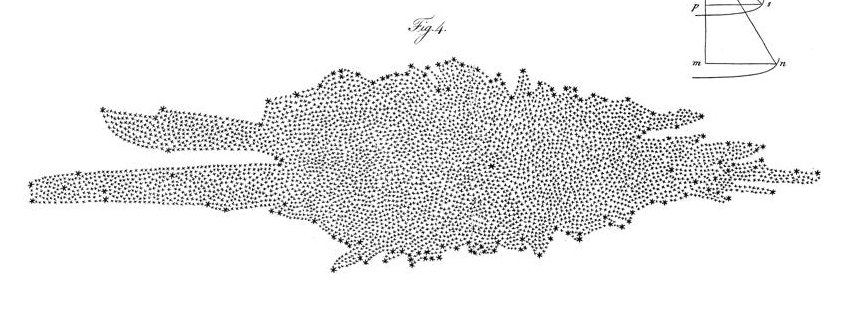
\includegraphics[width=1.0\textwidth]
	{./figures/1_introduction/Herschel_Model.png}
	
	\caption{\small{Modelo de William Herschel para nuestra galaxia, basado
	en un conteo de estrellas y la asunción de igual luminosidad 
	\cite{Herschel1785}.}}
	
	\label{fig:HerschelModel}
\end{figure}
%.........................................................................


Otra importante cuestión observacional que estaba emergiendo en esa época
fue sobre la existencia de otros \textit{universos islas} tal como el nuestro.
Era ya bien conocida la existencia de cuerpos extendidos en el cielo que no
se acomodaban satisfactoriamente a la definición de estrellas o planetas,
tales como nebulosas, discos planetarios y galaxias. Incluso William Herschel
y su hijo John Herschel contribuyeron con la realización de un gran catálogo
(para la época) de cuerpos extendidos conocido como \textit{Catálogo de 
Nebulosas y Cúmulos de Estrellas} y una versión extendida terminada por
John Dreyer en 1888, \textit{Nuevo Catálogo General de Nebulosas y Cúmulos
de Estrellas}, los cuales junto con el \textit{Índice de Catálogos} de 
1895 y 1908 constituyen una amplia colección de cuerpos ampliamente usados
en la astronomía actual, referidos con sus abreviaciones en inglés \textit{NGC}
y \textit{IC} respectivamente \cite{longair2008}. A pesar de todos estos
logros observacionales, la naturaleza real de estos objetos era un completo 
misterio, especialmente si ellos eran objetos dentro de nuestra propia 
galaxia o eran sistemas completamente independientes.


Esta última cuestión permaneció hasta el siglo veinte, y junto con el tamaño
real del universo constituyeron los dos grandes temas tratados en el 
conocido \textit{Gran Debate}, también denominado \textit{Debate de 
Shapley-Curtis}. Un importante evento en la historia de la astronomía donde
los astrónomos Harlow Shapley y Herber Curtis sometieron respectivamente 
diferentes argumentos a favor y en contra de la pertenencia de esos objetos
a nuestra galaxia y si la Vía Láctea era todo nuestro universo 
\cite{Curtis1921} \cite{Shapley1921}. A pesar de todo, sus argumentos fueron 
poco concluyentes y la solución a estos problemas debió esperar hasta 1924 
cuando Edwin Hubble midió la distancia a la galaxia de Andrómeda (M31 o 
NGC 224) y demostró incuestionablemente la verdadera naturaleza extragaláctica 
de este objeto, y en años posteriores para los demás \cite{Hubble1926}. 
Este logro junto con la verificación observacional de la expansión del 
universo (también debida a Hubble) fueron el comienzo de la cosmología 
observacional moderna.


También sucedió en este mismo siglo un evento clave para las modernas 
\textit{ciencias de la gravedad}, Albert Einstein formuló su Teoría
General de la Relatividad \cite{Einstein1916}, cambiando completamente 
la concepción previa de espacio y tiempo y llegando así a nuestro paradigma 
cosmológico actual.


%*************************************************************************




%*************************************************************************
%The current cosmology picture
\section{El Paradigma Cosmológico Actual}
\label{sec:TheCurrentCosmologyPicture}


Las bases teóricas para la relatividad general comenzaron a surgir con el 
auge de las geometrías no Euclidianas en el siglo diecinueve y comienzos 
del veinte, cuando fue demostrado que el quinto postulado de Euclides no 
era necesario para construir geometrías autoconsistentes y llegando así a 
las geometrías no planas (ver figura \ref{fig:NonEuclidean}). En especial 
fueron destacables los trabajos de Nikolai Lobachevsky (padre de las 
geometrías no Euclideas) y Bernhard Riemman, fundador de la geometría 
Riemanniana.


%.........................................................................
%Herschel Model of Our Galaxy
\begin{figure}[htbp]
	\centering
	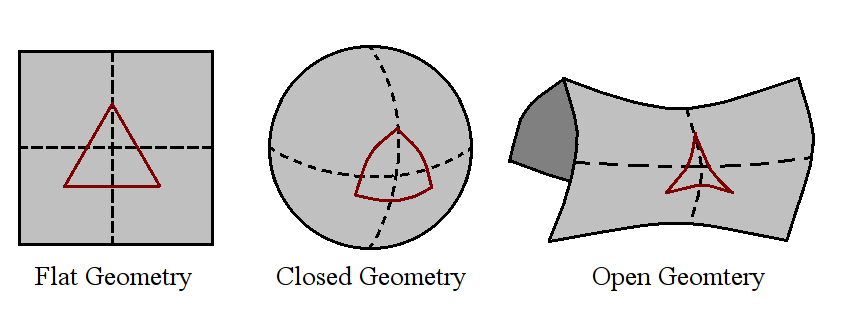
\includegraphics[width=0.9\textwidth]
	{./figures/1_introduction/Non_Euclidean.png}
	
	\caption{\small{Diferentes geometrías con variación del quinto postulado 
	de Euclides.}}
	
	\label{fig:NonEuclidean}
\end{figure}
%.........................................................................


A pesar de que estos primeros desarrollos en geometría habían dado lugar a
fuertes discusiones sobre el tipo de geometría del universo, los conceptos 
de espacio y tiempo eran aún interpretados de forma absoluta y más aún, su 
conexión con la gravedad completamente ignorada. Es por esta razón que 
la formulación de la Relatividad General abrió la puerta a toda nuestra
comprensión moderna.


Una vez obtenidas las ecuaciones de campo métrico de la Relatividad General
fue posible construir modelos globales y autoconsistentes del universo. Un
primer intento se debe al propio Einstein, quién formuló con influencia 
de su propia creencia un modelo de universo estático y cerrado. Para lograr 
esto debió hacer uso de la bien conocida constante cosmológica para 
contrarrestar la expansión/contracción natural de las soluciones que da
la teoría.


Pocos años después Aleksander Friedmann demostró en una serie de dos 
artículos un conjunto de soluciones para universos cerrados o hiperbólicos
que se expanden desde una singularidad \cite{FriedmanA} \cite{FriedmanB}, 
lo que concordaba perfectamente con las observaciones realizadas por Hubble 
para el corrimiento al rojo de galaxias distantes. Debido a esto, la 
inclusión de la constante cosmológica para soluciones estacionarias es 
conocido históricamente y reconocido por él mismo, como el mayor ‘‘resbalón’’ 
de la vida de Einstein. Después de esto hubo un aumento considerable en las 
investigaciones sobre la naturaleza del universo acorde a este tipo de 
soluciones, como la dinámica a gran escala, la geometría global y la 
medición precisa de un conjunto de parámetros cosmológicos de los modelos.


El siguiente avance importante viene con la formulación de la teoría del 
Big Bang por parte de George Gamow, donde se propone que los primeros
estadios del universo habían sido muy densos y calientes, partiendo de una
singularidad y llegando a los estadios tardíos donde el universo se ha 
estado expandiendo y enfriando, acorde a la solución de Friedmann. Una
de las primeras consecuencias de esta teoría es la nucleosíntesis temprana,
donde reacciones de fusión de hidrógeno produjeron elementos más pesados 
a partir del Hidrógeno, tales como Helio y Litio, lo cual no puede ser 
explicado a partir de reacciones de fusión en estrellas. La nucleosíntesis
temprana fue demostrada por Ralph Alpher y Robert Herman y ha sido 
corroborada observacionalmente de forma muy precisa.

\
%.........................................................................
%Cosmic Background Radiation
\begin{figure}[htbp]
	\centering
	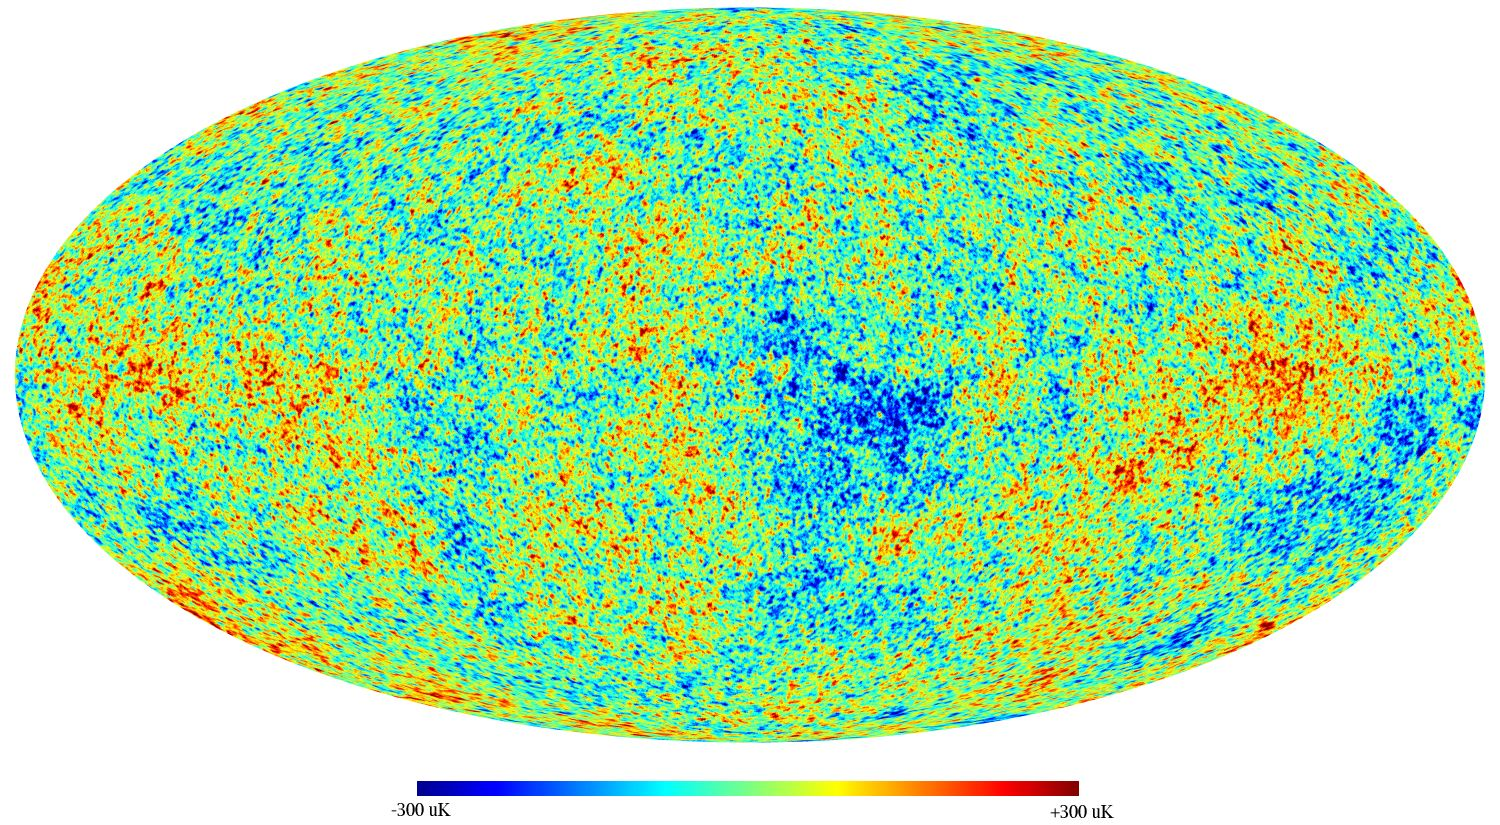
\includegraphics[width=0.8\textwidth]
	{./figures/1_introduction/CMB.png}
	
	\caption{\small{Radiación cómica de fondo. Tomado de 
	\url{http://upload.wikimedia.org/wikipedia/commons/3/3c/Ilc_9yr_moll4096.png}}}
	
	\label{fig:CMB}
\end{figure}
%.........................................................................


La segunda consecuencia del Big Bang es la presencia de un remanente de 
radiación de cuerpo negro del universo temprano, donde debido a la alta 
densidad y temperatura este era dominado completamente por la radiación.
Esto fue corroborado por observacionalmente por Arno Penzias y Robert
Wilson en 1965 con el descubrimiento de la radiación cósmica de microondas
(CBM por su siglas en inglés), donde se midió un espectro de cuerpo negro
de fondo en el universo con una temperatura asociada de $T = 2.725$ K. 
Estas dos predicciones de al teoría del Big Bang han hecho que sea 
adoptado como parte del modelo cosmológico estándar.


Uno de los primeros problemas originados con el descubrimiento de la 
radiación cósmica de fondo es el problema de horizonte. Esto surge debido
la alta isotropía angular medida en el espectro de radiación de fondo (ver 
figura \ref{fig:CMB}), indicando una conexión causal entre regiones tan 
apartadas del universo, que en principio no deberían estarlo. La solución 
al problema fue propuesta por Alan Guth en 1980 y se denomina teoría de 
inflación. En esta se postula una expansión exponencial en el universo 
temprano impulsada por un campo escalar (inflatón). En este periodo de 
expansión se magnificaron las fluctuaciones cuánticas del vacío de todos 
los campos presentes en el universo, produciendo así pequeñas perturbaciones 
en el campo de densidad de las cuales luego evolucionarían las estructuras 
a gran escala de la actualidad. Acorde a esto, la teoría inflacionaria 
también explica satisfactoriamente el problema de pequeñas perturbaciones 
en el universo primigenio, convirtiéndose así en parte del paradigma 
cosmológico actual.


La existencia de la materia oscura fue propuesta desde principios de la 
década de 1930, primero por parte de Jan Oort en 1932 y luego por Fritz
Zwicky en 1933, para dar cuenta de materia no lumínica en galaxias y 
cúmulos galácticos que se manifiesta de forma dinámica. A pesar de esto 
su naturaleza física era completamente desconocida. En 1984 Joel Primack,
George Blumenthal, Sandra Moore y Martin Rees propusieron un modelo de 
materia oscura fría (CDM por sus siglas en inglés), para el cual la 
materia oscura corresponde a un tipo de partícula no relativista que solo
interactua gravitacionalmente y de forma muy débil electromagnéticamente.
Bajo este esquema es posible demostrar que la formación de estructuras a 
gran escala se da de forma jerárquica en un proceso de \textit{top-down},
en el cual las estructuras más pequeñas se forman primero y a partir de 
agrupación de estas se forman las estructuras de gran escala, lo que ha 
sido verificado observacionalmente por surveys de galaxias (ver sección
\ref{sec:CosmologicalObservations}).


En la década de 1990 algunas observaciones cosmológicas comenzaron a 
mostrar una rata de expansión acelerada para el universo, lo que solo 
puede ser explicado (ver subsección \ref{subsec:SimpleSolutionsOfTheUniverse})
con la inclusión de una constante cosmológica en las ecuaciones de campo
de la relatividad general. El término de energía oscura fue acuñado debido 
a que esta constante puede tomarse como una densidad física de energía que
actúa con una presión negativa, impulsando así la rata de expansión del 
universo, a pesar de esto su naturaleza física es completamente incierta.
Mediciones precisas muestran que actualmente el universo está dominado por 
este tipo energía, alcanzando el $70 \%$ del total de materia-energía 
presente en el universo. Eso último completa el paradigma cosmológico 
actual y es denominado modelo estándar $\Lambda$CDM o modelo de 
concordancia.

\
%.........................................................................
%Local Group
\begin{figure}[htbp]
	\centering
	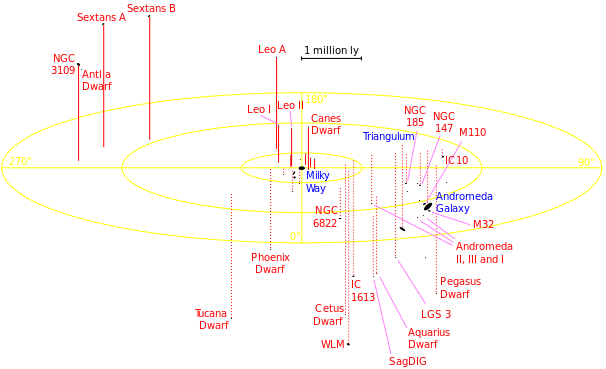
\includegraphics[width=1.0\textwidth]
	{./figures/1_introduction/LocalGroup.png}
	
	\caption{\small{Grupo Local. Tomado de 
	\url{http://commons.wikimedia.org/wiki/File:Local_Group.svg}}}
	
	\label{fig:LocalGroup}
\end{figure}
%.........................................................................


El grupo local es un sistema de aproximadamente 30 galaxias que interactúan
gravitacionalmente entre ellas y evolucionan de forma relativamente aislada
de otras estructuras a gran escala, con la Vía Láctea y Andrómeda como 
miembros más representativos (ver figura \ref{fig:LocalGroup}).


La importancia del grupo local en un contexto cosmológico se debe a que es
la estructura a gran escala más conocida, permitiendo así verificar las 
predicciones del modelo cosmológico estándar. Entre los problemas actuales
en esta línea destacan la sobreabundancia de galaxias satélites para la 
Vía Láctea, la conexión entre los flujos de las nubes de Magallanes y la
galaxia de Andrómeda, fuerzas de marea en el grupo local, la cinemática 
de Andrómeda y la Vía Láctea en un contexto cosmológico \cite{forero2013}
y la influencia del entorno cosmológico en la formación de sistemas como
el grupo local.


%*************************************************************************





%*************************************************************************
%Cosmological observations
\section{Observaciones Cosmológicas}
\label{sec:CosmologicalObservations}
	

El auge generado por la era espacial junto con el gran avance tecnológico
de ins\-trumentos de medida y sensores ha potenciado enormemente las 
investigaciones observacionales en cosmología, permitiendo en conjunto con 
los avances teóricos llegar al paradigma cosmológico actual y contrastar los 
diferentes modelos que han surgido. A continuación se presentan algunos de 
los proyectos observacionales más destacados en cosmología y que son 
ampliamente usados en investigaciones actuales.


	%---------------------------------------------------------------------
	%2DF Galaxy Redshift Survey
	\subsection*{2DF Galaxy Redshift Survey}
	\label{subsec:2DFGRS}
	%---------------------------------------------------------------------
	
	
El 2DF Galaxy Redshift Survey (2DFGRS) o sondeo de corrimiento al rojo en 
un campo de 2 grados\footnote{Página oficial del proyecto 
\url{http://magnum.anu.edu.au/~TDFgg/}.}, es un sondeo del corrimiento al 
rojo de un conjunto de galaxias dentro de una área de $1500$ grados cuadrados 
para zonas cercanas al polo sur y norte galáctico esto para evitar la extinción 
provocada por el disco galáctico. Fue realizado por el telescopio de $3.9$ m 
del observatorio Anglo-Australiano entre 1997 y 2002. Entre los principales 
resultados de este sondeo destaca el establecimiento de la estructura local 
a gran escala en torno al grupo local a partir de medidas fotométricas de 
$382\ 323$ objetos para corrimientos al rojo menores a $z=0.3$, también 
destaca la medida del parámetro de densidad de materia no relativista (
oscura + bariónica) en el modelo cosmológico estándar.

	
	%---------------------------------------------------------------------
	%Sloan Digital Sky Survey
	\subsection*{Sloan Digital Sky Survey}
	\label{subsec:SDSS}
	%---------------------------------------------------------------------


El Sloan Digital Sky Survey (SDSS) o sondeo digital del espacio Sloan, al 
igual que el 2DFGRS es un sondeo en corrimiento al rojo del universo a 
gran escala realizado por el telescopio de $2.5$ m en el observatorio Apache 
Point en Nuevo México desde el año 2000.


%.........................................................................
%SDSS
\begin{figure}[htbp]
	\centering
	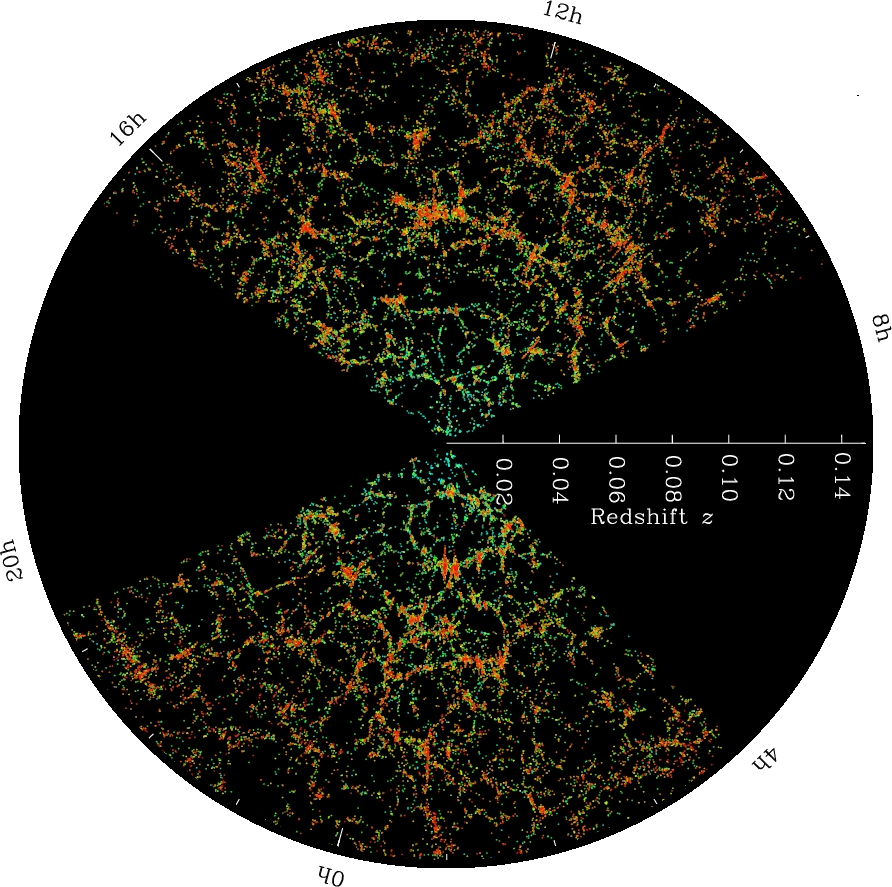
\includegraphics[width=0.6\textwidth]
	{./figures/1_introduction/SDSS.png}
	
	\caption{\small{Mapa del universo a gran escala de acuerdo al Sloan 
	Digital Sky Survey. Tomado de la página oficial del proyecto 
	\url{http://www.sdss.org/}}}
	
	\label{fig:SDSS}
\end{figure}
%.........................................................................


El sondeo cubre una zona significativamente mayor que el 2DFGRS, 
aproxi\-madamente $7500$ grados cuadrados y ha catalogado alrededor de 
$2$ millones de objetos, permitiendo construir un mapa a gran escala del 
universo y percibir por primera vez la estructura de la red cósmica 
(ver figura \ref{fig:SDSS}).
	
	
	%---------------------------------------------------------------------
	%WMAP
	\subsection*{WMAP}
	\label{subsec:WMAP}
	%---------------------------------------------------------------------


La Wilkinson Microwave Anisotropy Probe (WMAP), es una sonsa espacial de 
la NASA lanzada en 2001 y ubicada en el punto de Lagrange L2. Su principal 
objetivo es medir con muy alta precisión los pequeños contrastes de 
temperatura y la polarización de la radiación cósmica de fondo (ver figura 
\ref{fig:CMB}). Aproximadamente cada 2 años la NASA libera los resultados
acumulados obtenidos, referidos como WMAP1, WMAP3, WMAP5, WMAP7 y 
finalmente en el 2012 el WMAP9. Los resultados obtenidos por el WMAP han 
sido hasta el momento la prueba más fehaciente del modelo cosmológico 
estándar $\Lambda$CDM. En especial destacan la medida precisa de la edad del
universo, los diferentes parámetros de densidad, la constante de Hubble, 
la determinación de la geometría global del universo (plana) y la 
confirmación del modelo inflacionario.

\
%.........................................................................
%Cosmological Parameter of WMAP7
\begin{table}[htbp]
\begin{small}
\centering
\begin{tabular}{|c|c|c|c|} \hline
\cellc{\textbf{Parámetro}}		&
\cellc{\textbf{Notación}}		&  
\cellc{\textbf{Valor}}			& 
\cellc{\textbf{Unidades}}					\\ \hline


Edad del Universo  			&	$t_0$			&	$13.75 \pm 0.13$	&	Ga 			\\ \hline

Constante de Hubble			&	$H_0$			&	$71.0 \pm 2.5$		&   km/(Mpc s)	\\ \hline

Parámetro de Hubble			&	$h$				&	$0.71 \pm 0.025$	&   --			\\ \hline

Densidad de Bariones		&	$\Omega_b$		&	$0.0449\pm 0.0027$	&	--			\\ \hline

Densidad de & & & \\
Materia Oscura				&	$\Omega_c$		&	$0.222 \pm 0.026$	&	--			\\ \hline

Densidad de & & & \\
Energía Oscura				&	$\Omega_\Lambda$&	$0.734 \pm 0.029$	&	--			\\ \hline

Densidad de & & & \\
Radiación					&	$\Omega_r$		&$8.24 \times 10^{-5}$	&	--			\\ \hline

Amplitud de & & & \\
Fluctuaciones en $8h^{-1}$ Mpc&	$\sigma^2_8$	&	$0.801 \pm 0.030$	&	--			\\ \hline

Índice Espectral			&	$n_s$			&	$0.963 \pm 0.014$	&	--			\\ \hline
Profundidad Óptica & & & \\
de Reionización 			&	$\tau$			&	$0.088 \pm 0.015$	&	--			\\ \hline
				
Densidad Total & & & \\
del Universo	&	$\Omega_0$		&	$1.080\ \mbox{\scriptsize{$+0.093$}}/ 
										\mbox{\scriptsize{$-0.071$}} $&	--				\\ \hline
\end{tabular}
\caption{Parámetros cosmológicos WMAP7 \cite{WMAP7}.}
\label{tab:CosmologicalParameters}
\end{small}
\end{table}
%.........................................................................


En la tabla \ref{tab:CosmologicalParameters} se tabulan los resultados 
del WMAP7 \cite{WMAP7}, los cuales son ampliamente usados en los siguientes 
capítulos y en especial las diferentes simulaciones cosmológicas presentadas en
los capítulos \ref{cha:N-BodySimulations} y \ref{cha:Results} están basadas
en estos.


%*************************************************************************

%---------------------- Theoretical Frame -----------------------

%qqqqqqqqqqqqqqqqqqqqqqqqqqqqqqqqqqqqqqqqqqqqqqqqqqqqqqqqqqqqqqqqqqqqqqqqq
%Quote
%\begin{savequote}[50mm]
%‘‘El cosmos es todo lo que es, todo lo que fue y todo lo que será. Nuestras 
%más ligeras contemplaciones del cosmos nos hacen estremecer: Sentimos como 
%un cosquilleo nos llena los nervios, una voz muda, una ligera sensación como
%de un recuerdo lejano o como si cayéramos desde gran altura. Sabemos que nos
%aproximamos al más grande de los misterios.’’
%\qauthor{Carl Sagan}
%\end{savequote}
%qqqqqqqqqqqqqqqqqqqqqqqqqqqqqqqqqqqqqqqqqqqqqqqqqqqqqqqqqqqqqqqqqqqqqqqqq




%#########################################################################
\chapter{Cosmología y Formación de Estructuras.}
\label{cha:Theoretical Framework}

\section{Relatividad General en el ámbito cosmológico (Universo homogéneo e isótropo )}
\label{sec:IsotropicAndHomogeneousUniverse}
%***********************************************************************
En la naturaleza existen cuatro fuerzas fundamentales. Al considerar un sistema donde interactúan  dos ó más cuerpos con masa, la fuerza que intermedia entre las partículas  es la fuerza de la gravedad. Es por eso que cuando se pretende abordar el estudio de la dinámica de este tipo de interacciones se debe remitir a la teoría de la gravedad. En la actualidad la mejor forma de reproducir la dinámica del universo es haciendo uso de la teoría de la Relatividad de Albert Einstein.
%Cuando se pretende estudiar el funcionamiento del universo en general, se debe invocar la ciencia que se encarga de ello. La cosmología estudia la dinámica del universo, el origen, evolución y futuro del mismo.  %Cuando se introducen la teoría de la relatividad general esta empieza a ser parte de la física, pues las leyes que describen el universo como un todo son las mismas que determinan el funcionamiento de los sistemas que se encuentra adentro de él. Esta teoría se  sustenta por una base matemáticamente robusta que  puede predecir eventos y reproduce las observaciones. 

En el camino de poder estudiar la dinámica del universo, un  paso obligado es conocer las ecuaciones de Einstein y poder ende conocer sus soluciones, que son de gran importancia, porque relaciona la estructura del espacio-tiempo con su contenido de materia y su energía. 
%Estas ecuaciones no pueden dar una solución general exacta, es entonces necesario introducir ....
La cosmología pretende  describir el funcionamiento del universo a muy grandes escalas, donde al despreciar las contribuciones de las galaxias, estrellas y otros objetos es posible obtener solución a las ecuaciones de Einstein.

Aunque la cosmología pueda describir los eventos a grandes escalas es necesario partir de algo, introducir restricciones que permitan reproducir el universo actual. Es por esto, que la cosmología parte de dos principios fundamentales:  

- El primer principio cosmológico, habla sobre la distribución de la materia y la forma del universo a medida que evoluciona. Si se toma un punto cualesquiera en el espacio, la distribución  alrededor de él es invariante en el tiempo, sin importar la dirección en la cual se observe. Una forma más estricta de decir este principio es:\\

{\bf{Principio cosmológico:}} {\textit{El cualquier momento, el universo es homogéneo e isótropo a muy grandes escalas.}} (Bert Janssen,2013,p. 207). \\

Cuando se cuenta con un espacio el cuál es homogéneo e isótropo este espacio presenta un máximo de simetría.  Matemáticamente, nos dice que la métrica es invariante bajo cualquier rotación o traslación. 

?`Qué tan cierto puede llegar a ser esto? ?` el universo sí es homogéneo e isótropo ? Cuando se observa el universo, la materia tiende a estar concentrada, las estrellas se concentran en galaxias, las galaxias en cúmulos de galaxias y a su vez estos cúmulos en otros súper cúmulos. Entonces, ?`que tan cierto es que el universo sea homogéneo? Para tener un universo homogéneo e isótropo se debe considerar observaciones a una escala mucho mayor (en el orden de $10^{9}$ años luz), un ejemplo es la radiación cósmica de fondo, que corresponde a la radiación térmica proveniente del origen del universo, la cual tiene una anisotropía del orden de $\Delta T /T \approx= 10^{-5}$. 

- El segundo principio cosmológico trata sobre la dinámica de las sobre densidades en el universo, el cual enuncia que el  movimiento es despreciables cuando se compara con el movimiento cosmológico. El segundo principio se denomina como Postulado de Weyl el cual dice: \\

{\bf{Postulado de Weyl:}} {\textit{La materia a escalas cosmológicas se comporta como un fluido perfecto, cuyas componentes se mueven a lo largo de geodésicas temporales, que no se intersectan, salvo (posiblemente) en un punto en el pasado.}} (Bert Janssen,2013,p. 209)\\

El postulado de Weyl implica una idea muy importante en la cosmología, los observadores privilegiados. Estos observadores  se encuentran en reposo con respecto al fluido, lo cual implica que su movimiento es con respecto a la evolución del universo. El nombre que se le dan a estos observadores son los observadores comóviles. Cuando se define este tipo de observadores también se define un tiempo cosmológico, que corresponde a la dirección temporal del observador comóvil. 



%*************************************************************************
%Geometría
\section{Geometría}
\label{sec:Geometría}
%***********************************************************************

%---------------------------------------------------------------------
	%Metrica
	\subsection{Métrica}
	\label{subsec:Metrica}
	%---------------------------------------------------------------------
	
En la relatividad general la métrica permite definir distancias, ángulos y volúmenes en un espacio Euclideo. Además juega un papel importante porque convierte las coordenadas dependientes del observador $X^{\mu}=(t,x^{i})$ en elementos de línea invariante


\begin{equation}
ds^{2}=\sum_{\mu,\nu}^{4} g_{\mu\nu}dX^{\mu}dX^{\nu} \equiv g_{\mu\nu}dX^{\mu}dX^{\nu} \,.
\label{eq:tensor_metrico}
\end{equation}

La métrica tiene una dependencia espacial y temporal $g_{\mu\nu}(t,{\bf{x}})$, entonces dependerá de donde se esté tomando y en que momento. Por esta dependencia espacio-temporal la métrica también dependerá de la distribución de la materia y la energía, debido a que esta debe reproducir los efectos de la gravedad.

La elección de la métrica responde al universo que se quiere. Para un universo homogéneo e isótropo se puede considerar un sistema con simetría esférica. La expresión para describir el diferencial de longitud entre dos puntos sobre la superficie de una esfera se escribe de la forma

\begin{equation}
dl^{2}=R_{c}^{2}d\theta^{2}+R_{c}^{2}\sin^{2}\theta d\phi^{2} \,,
\label{metrica_esfera}
\end{equation}
%
donde $R_{c}$ es el radio de curvatura de la esfera. La figura (\ref{fig:diferencial_linea_esferico}) presenta el diferencial de línea para una simetría esférica.


%------------------------------------------------------
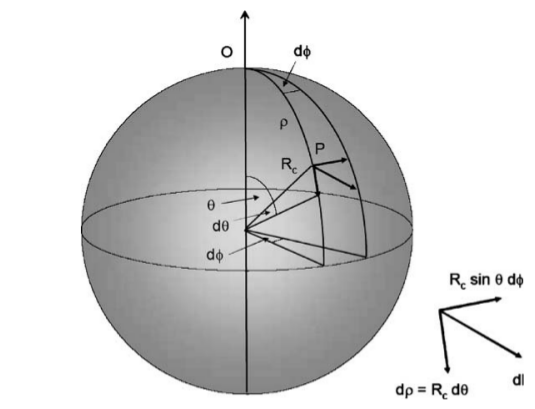
\includegraphics[scale=.4]{./figures/2_theoretical_framework/diferencial_linea.png}
\figcaption{\emph{Representación del diferencial de línea para simetría esférica.}}\label{fig:diferencial_linea_esferico}


%------------------------------------------------------

Usando la figura (\ref{fig:diferencial_linea_esferico}) se construye un arco $\rho$ entre los puntos O y P cuya distancia es $\rho=\theta R_{c}$, entonces la ecuación (\ref{metrica_esfera}) puede reescribirse de la forma

\begin{equation}
dl^{2}=d\rho^{2}+R_{c}^{2}\sin^{2}\left(\frac{\rho}{R_{c}} \right)d\phi^{2} \,.
\end{equation}
%
Una forma alternativa de escribir la métrica es introduciendo una distancia

\begin{equation}
x=R_{c}\sin\left(\frac{\rho}{R_{c}} \right) \,.
\end{equation}
%
Al calcular el diferencial y elevando al cuadrado se obtiene
%
\begin{equation}
dx^{2}=\left[1-\sin^{2}\left( \frac{\rho}{R_{c}}\right) \right]d\rho^{2}  \,, \hspace{1cm} d\rho^{2}=\frac{d^{2}}{1-kx^{2}} \,,
\end{equation}
%
donde $k=1/R_{c}^{2}$ es el parámetro de curvatura.

Por lo tanto la métrica se puede escribir de la forma 

\begin{equation}
dl^{2}=\frac{dx^{2}}{1-kx^{2}}+x^{2}d\phi^{2} \,.
\end{equation}

Se debe recordar que la constante de curvatura $k$ puede representar tres tipos de geometrías: Cuando se tiene una curvatura positiva se obtiene simetría esférica cerrada, con curvatura cero se obtiene el espacio Euclideo plano y si es negativo se tiene una geometría hiperbólica abierta. Ver figura (\ref{fig:curvatura_k}).\\

%-----------------------------------------
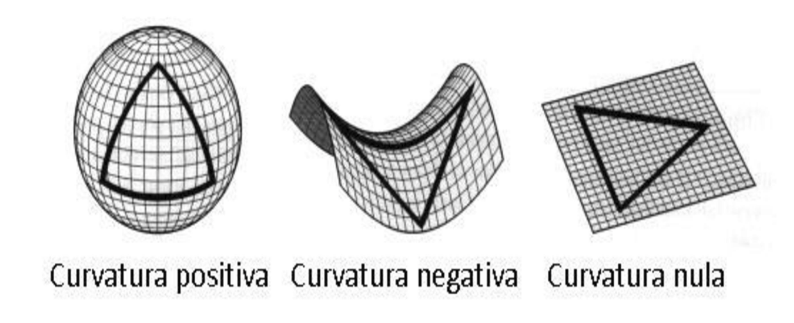
\includegraphics[scale=.4]{./figures/2_theoretical_framework/curvatura_k.png}
\figcaption{\emph{Tres espacios con curvatura constante, esfera con curvatura positiva (izquierda), hiperboloide con curvatura negativa (centro) y plano con curvatura cero (derecha)}.}\label{fig:curvatura_k}

%--------------------------------------------

Extrapolando el diferencial de linea a tres dimensiones en termino de las coordenadas polar esférica $(\rho, \theta, \phi)$ se llega a 

\begin{equation}
dl^{2}=d\rho^{2}+R^{2}_{c}\sin^{2}\left(\frac{\rho}{R_{c}}\right)[d\theta^{2}+\sin^{2}\theta d\phi]\,,
\end{equation}
%
y como se hizo anteriormente también se puede llegar a la ecuación en termino de $x, \theta, \phi$

\begin{equation}
dl^{2}=\frac{x^{2}}{1-kx^{2}}+ x^{2}[d\theta^{2}+\sin^{2}\theta d\phi]\,.
\end{equation}
%
Ahora se puede dar el salto de escribir la métrica considerando el tiempo y llegar a una métrica espacio-temporal

\begin{equation}
ds^{2}=dt^{2}-\frac{1}{c^{2}}dl^{2}\,.
\label{ec:metrica_general}
\end{equation}

Para un modelo isotrópico, se tiene una función que permite describir como cambia la distancia entre dos observadores cualesquiera en un instante de tiempo. $a(t)$ es conocido como el factor de escala y viene dada por 

\begin{equation}
\rho(t)=a(t)r\,,
\end{equation} 
%
r es llamada la \textit{ coordenada radial de distancia comóvil}. Se establece que $a(t)=1$ si $t=t_{o}$ que equivale al universo de hoy.\\

Llamando $R_{c}(t_o)$ como el radio de curvatura para la presente época entonces, $\Re$ se relaciona de la forma

\begin{equation}
R_{c}=a(t)\Re \,.
\end{equation}
%
Sustituyendo $\rho$ y $R_{c}$ en la métrica (\ref{ec:metrica_general}) y considerando $d\Omega^{2}=d\theta^{2}+\sin^{2}\theta d\phi^{2}$ se obtiene 

\begin{equation}
ds^{2}=dt^{2}-\frac{a^{2}(t)}{c^{2}}[dr^{2}+\Re^{2}\sin^{2}(r/\Re)d\Omega^{2}]\,.
\end{equation}
%
Esta es la métrica de Robertson-Walker. Es importante notar que $a(t)$ describe la dinámica del universo y $\Re$ describe la curvatura espacial del universo en la presente época.

Otra forma de representar la métrica es usando \textit{diametro angular comóvil} $r_{1}=\Re\sin(r/\Re)$

\begin{equation}
ds^{2}=dt^{2}-\frac{a^{2}(t)}{c^{2}}\left[\frac{dr^{2}_{1}}{1-kr^{2}_{1}}+r^{2}_{1}d\Omega^{2}\right]\,,
\end{equation}
%
donde $k=1/\Re^{2}$.

Retomando la ecuación inicial (\ref{eq:tensor_metrico}), el tensor métrico $g_{\mu\nu}$ sería


%\begin{bmatrix}
%1 & 0 & 0 & 0\\ 
%0 & $\frac{-a^{2}(t)}{1-kr^{2}}}$ & 0  & 0\\ 
%0 & 0 & $-a^{2}(t)^{2} $  & 0 \\ 
%0 & 0 & 0 & $-a^{2}(t)\sin^{2}(\theta)$
%\end{bmatrix}


\begin{equation}
g_{\mu\nu}=
\begin{bmatrix}
1 & 0 & 0 & 0 \\ 
0 & \frac{-a^{2}(t)}{1-kr^{2}} & 0 & 0 \\ 
0 & 0 & -a^{2}(t)  & 0 \\ 
0 & 0 & 0 & -a^{2}(t)\sin^{2}(\theta)
\end{bmatrix}\,.
\end{equation}


%\newpage
%*************************************************************************
%The Friedmann equations
\section{Ecuaciones de Friedmann}
\label{sec:Ecuaciones_Friedmann}
%************************************************************************

En Relatividad General, las ecuaciones de campo de Einstein brindan información muy importante sobre la relación entre la energía, masa y la geometría del espacio-tiempo, cuya relación es dada por 

\begin{equation}
R_{\mu\nu}-\frac{1}{2}R-g_{\mu\nu}\Lambda=\frac{8\pi G}{c^{4}}T_{\mu\nu} \,,
\label{eq:Einstein_campo_ecuacion}
\end{equation}
%
donde $R_{\mu\nu}$ es el tensor de Ricci, $R$ es el escalar de Ricci, $g_{\mu\nu}$ es la métrica, $\Lambda$ constante cosmológica y $T_{\mu\nu}$ es el tensor momentum-energía. 

El tensor y escalar de Ricci se pueden calcular de la siguiente manera

\begin{eqnarray}
R_{\mu\nu} \equiv \partial_{\lambda}\Gamma^{\lambda}_{\mu\nu} - \partial_{\nu}\Gamma^{\lambda}_{\mu\lambda} + \Gamma^{\lambda}_{\lambda\rho} \Gamma^{\rho}_{\mu\nu} - \Gamma^{\rho}_{\mu\lambda} \Gamma^{\lambda}_{\nu\rho}\,,
\end{eqnarray}

\begin{equation}
R=R^{\mu}\,_{\mu}=g^{\mu\nu}R_{\mu\nu}\,,
\label{eq:Tensor_Ricci}
\end{equation}
%
donde 

\begin{equation}
\Gamma^{\nu} \,_{\alpha\beta}=\frac{1}{2}g^{\mu\sigma}(\partial_{\beta} g_{\sigma\alpha}+\partial_{\alpha} g_{\sigma\beta}-\partial_{\sigma} g_{\alpha\beta})\,.
\end{equation}

Debido a la isotropía del espacio en la métrica de \textit{Robertson-Walker}, no es necesario calcular las componentes $R_{i0}=R_{oi}$. Las componentes que no se hacen cero del tensor de Ricci son


\begin{eqnarray}
R_{00}=-3\frac{\ddot{a}}{a}\,, \hspace{2cm} \\
R_{ij}=-\left[\frac{\ddot{a}}{a}+ 2\left(\frac{\dot{a}}{a}\right)^{2} + 2\frac{k}{a^{2}} \right]g_{ij} \hspace{1cm} i,j=0,1,2\,,
\end{eqnarray}

\begin{align}
R_{\mu\nu}=R_{00}+R_{ij}\,,
\label{eq: tensor_Ricci}
\end{align}

y el escalar de Ricci queda 

\begin{equation}
R=-6\left[\frac{\ddot{a}}{a} + \left(\frac{\dot{a}}{a} \right) + \frac{k}{a^{2}} \right]\,.
\label{eq:Ricci_escalar}
\end{equation}

En cosmología cuando se pretende calcular el tensor momentum-energía, se considera  un fluido perfecto. Tomando el tensor como la suma de sus componentes $T_{\mu\nu}=T_{ij}+T_{i0}+T_{0j}+T_{00}$, y debido a la isotropía se tiene que $T_{i0}=T_{0j}=0$. Al considerar entonces la isotropía y la homogeneidad se tiene

\begin{equation}
T_{00}= \rho(t)\,, \hspace{1cm} T_{io}=0\,, \hspace{1cm} T_{ij}=-P(t)g_{ij}(t,\bf{x})\,.
\label{eq: Tensor_momentum-energia}
\end{equation}
%
Remplazando (\ref{eq: Tensor_momentum-energia}), (\ref{eq:Ricci_escalar}) y (\ref{eq: tensor_Ricci}) en la ecuación (\ref{eq:Einstein_campo_ecuacion}), se permiten llegar a dos ecuaciones escalares acopladas

\begin{equation}
\frac{\ddot{a}}{a} = -\frac{4\pi G}{3}\left(\rho + \frac{3P}{c^{2}} \right) + \frac{c^{2}\Lambda}{3}\,,
\end{equation}
\begin{equation}
\frac{\ddot{a}}{a}+2 \left(\frac{\dot{a}}{a}\right)^{2} + 2k\left(\frac{c}{a} \right)^{2} =4\pi G\left( \rho - \frac{P}{c^{2}}\right)+ c^{2}\Lambda\,,
\end{equation}
%
donde $\rho$ es la densidad y $P$ es la presión.

La importancia de estas ecuaciones radica en que permiten conocer la evolución del universo (homogéneo e isótropo) usando el factor de escala. 


%*************************************************************************
%The Friedmann equations
\section{Formación de Estructuras.}
\label{sec:Estructure_Formation}
%************************************************************************



%Buscando poder demostrar un modelo que permita modelar la estructura del universo a gran escala, se hace uso de la {\it{Inestabilidad de Jeans}}. Esta teoría representa la evolución del universo, partiendo de los principios fundamentales (homogeneidad e isotrpía).

Al observar el universo a gran escala, es claro que posee alta simetría y homogeneidad, pero ?`qué pasa cuando se mira a escalas menores? A escalas menores que la cosmológicas, los sistemas son asimétricos e inhomogéneos, lo cual implica una alta complejidad. Por esto, es necesario realizar modelos que permitan reproducir lo observacional, asumiendo aproximaciones coherentes,  haciendo que el grado de dificultad disminuya. El universo a escalas menores que las cosmológicas, presenta no linealidad en casi todos sus sucesos; la formación de estructuras es un caso de ello. La forma de introducir la linealidad o no linealidad en la formación de estructuras es considerando el campo de densidad. Para él régimen lineal se supone ($\delta\rho << \bar{\rho}$), donde la perturbación de la densidad es mucho menor que la densidad media. Mientras que para el régimen no lineal se supone que la perturbación es aproximada a la densidad media ($\delta\rho \sim \bar{\rho}$).


Con el propósito de poder reconstruir la estructura del universo en cualquier instante $t$ se considera lo siguiente:

Al observar el pasado, se debe pensar que existieron pequeñas desviaciones en la homogeneidad en la materia. A medida que el tiempo pasa, estas desviaciones incrementan, debido a la fuerza gravitacional. Esto fue generando una acumulación de materia cada vez mayor, que desencadeno la formación de estructuras, y que dieron origen a las primeras galaxias. Las soluciones a las ecuaciones de Friedmann permiten incrustar las perturbaciones que dan origen a la formación de estructuras.

Se debe tener presente que la teoría del régimen lineal solo se cumple para desviaciones pequeñas, osea, para un universo muy joven. Para poder reproducir las estructuras del universo observable, es necesario considerar un teoría de régimen no lineal. 


%*************************************************************************
%The Friedmann equations
\subsection{Régimen Lineal Para la Formación de Estructuras.}
\label{subsec:Lineal_Estructure_Formation}
%************************************************************************


%---------------------------------------------------------------------
	%M
	\subsubsection{Régimen Newtoniano.}
	\label{subsubsec:Newtonian_Regimen}
	%---------------------------------------------------------------------


En el régimen lineal la perturbación en la métrica $g_{\mu\nu}$ y su fuente $T_{\mu\nu}$ se escriben de la forma

\begin{equation}
g_{\mu\nu} \Rightarrow g_{\mu\nu}+\delta g_{\mu\nu} \hspace{0.8cm} T_{\mu\nu} \Rightarrow T_{\mu\nu} +\delta T_{\mu\nu} \,.
\end{equation}
%
Al supone que las perturbaciones son pequeñas es posible linealizar la ecuación de Einstein 

\begin{equation}
\hat{\mathcal{L}}(g_{\mu\nu})\delta g_{\mu\nu} = \delta T_{\mu\nu} \,,
\end{equation}
%
donde $\hat{\mathcal{L}}$ es el operador diferencial lineal que depende del espacio-tiempo. 
 
Una forma simple de poder calcular la dinámica de las perturbaciones es infiriendo que el radio de la perturbación es menor al radio de Hubble. Al decir esto se puede obviar del caso relativista y considerarlo meramente Newtoniano. Al suponer esto, se puede considerar la materia del universo como un fluido Newtoniano que colisiona. Esto implica que es posible usar las ecuaciones de un fluido Newtoniano:

\begin{eqnarray}
\frac{\partial \rho}{\partial t} + \nabla\cdotp(\rho v) = 0\,, \hspace{1cm} Ecuacion\ de\ continuidad \\
\label{eq: Navier-Stoke1}
\frac{\partial v}{\partial t} +(v\cdot \nabla)v = -\frac{\nabla p}{\rho}- \nabla\Phi \,,  \hspace{0.5cm} Ecuacion\ de\ Euler\\
\label{eq: Navier-Stoke2}
\nabla^{2}\Phi = 4\pi G\rho\,. \hspace{1.3cm} Ecuacion\ de\ Poisson\\
\label{eq: Navier-Stoke3}
\end{eqnarray}

Al aplicar las pequeñas perturbaciones cuasiestáticas a la densidad ($\rho=\rho_{o}+\delta\rho$), velocidad ($v=\delta v$), presión ($p=p_{o}+\delta p$) y al potencial gravitacional ($\Phi=\Phi_{o}+\delta\Phi$). Se obtiene 

%\begin{subequations}
\begin{align}
\frac{\partial \delta\rho}{\partial t} + \rho_{o}\nabla\cdotp(\delta v) = 0\,,
\label{eq:Navier-stoke1_perturbation}
\end{align}
%----------------
\begin{align}
\frac{\partial \delta v}{\partial t} + \frac{1}{\rho}\left(\frac{\partial p}{\partial \rho} \right)\nabla \delta \rho+ \nabla\delta\Phi =0\,,
\label{eq:Navier-stoke2_perturbation}
\end{align}
%-------
\begin{align}
\nabla^{2}\delta\Phi - 4\pi G\delta\rho = 0\,.
\label{eq:Navier-stoke3_perturbation}
\end{align}	
%\end{subequations}

Ahora el propósito es poder resolver las ecuaciones con perturbaciones (\ref{eq:Navier-stoke1_perturbation}, \ref{eq:Navier-stoke2_perturbation}, \ref{eq:Navier-stoke3_perturbation}). Para ello  se puede suponer soluciones de ondas planas\footnote{Cuando se supone un universo plano, se consideró la aparición de las ondas planas}

\begin{equation}
\delta u_{i} = \delta_{i}e^{i\bf{k}\cdot \bf{r}}\,,
\end{equation}
%
donde $\delta u_{i}= \delta\rho, \delta v, \delta\Phi$ y se entiende que $\delta_{i}$ equivale a las amplitudes. Permitiendo facilidad en los cálculos. 
%%Mi propósito no es solucionar estas ecuaciones, solo pretendo mostrar que consideraciones se deben hacer para llegar a los resultados
~\\
Al considerar la inestabilidad gravitacional, se puede obtener unos resultados  interesantes sobre la formación de la estructura. Entonces considerando lo siguiente: 

Para un fluido homogéneo e isotrópico, Jeans dice que a medida que el sistema va evoluciona se van generando pequeños cambios en la densidad $\delta \rho$ y en la velocidad $\delta v$.

De igual manera Jeans plantea que la aparición de una inhomogeneidad en la distribución de materia $\delta\rho$  generará un cambio en la fuerzas que preservan la homogeneidad. Entonces si $\delta\rho>0 $  la fuerza de gravitación $F_{g}$(responsable del colapso) deberá ser mayor que la fuerza de presión $F_{p}$(responsable del no colapso), entonces   $F_{g}>F_{p}$. Esta ultima afirmación da la condición necesaria para la formación de estructuras. Usando esta idea se puede determinar el radio necesario para el cuál se cumple la desigualdad, también conocido como el radio de Jeans $\lambda$.  

\begin{eqnarray}
F_{g} \approx G\rho\lambda \ \ \  y \ \ \ F_{p}\approx\frac{v_{s}^{2}}{\lambda}\\
\lambda^{2} > \frac{v_{s}^{2}}{G\rho} \,,
\end{eqnarray}

de una forma similar se puede llegar al tiempo gravitacional de caída libre 

\begin{equation}
\tau_{f-f} \approx \frac{1}{(G\rho)^{1/2}}\,.
\end{equation}


%*************************************************************************
%The Friedmann equations
\subsection{Régimen no lineal Para la Formación de Estructuras.}
\label{subsec:non-Lineal_Estructure_Formation}
%************************************************************************

Cuando se observo el universo en sus etapas tempranas, antes de la era de la recombinación\footnote{Instante en el universo donde la temperatura bajo lo suficiente para poder permitir la combinación de los electrones con los nucleos generando los primeros átomos. Antes de este instante se conoce como la época dominada por la radiación, electrones y protones libres.}, se consideró que las fluctuaciones $\delta$  en la materia eran despreciables ($\delta \ll 1$). Esta suposición permite facilitar muchos cálculos, pero restringe el tiempo de evolución del universo. Sin embargo, si se pretende determinar la evolución y estructuras a escalas mayores como en la actualidad, donde $\delta \gg 1$, es necesario hacer uso de otro método que permita reconstruir la dinámica del universo. Para ello se hace uso del régimen no lineal. Cabe resaltar que esta técnica es altamente complicada donde es necesario hacer aproximaciones y muchas veces no es posible llegar a soluciones analíticas, por esto se hace uso de los métodos numéricos que permiten encontrar aproximaciones a las soluciones. 

En la actualidad existe una gran variedad de métodos que describen la formación no lineal. Un caso especial es la aproximación de Zeldovich, la cual es capaz de reproducir el régimen lineal, permitiendo usar una  expresión analítica y reduciendo la complejidad de los cálculos. Este método además reproduce de muy buena manera el universo observable actual.

%-----------------------------------------
%\includegraphics[scale=.4]{./figures/2_theoretical_framework/Zeldovich.gif}
%\figcaption{\emph{Tres espacios con curvatura constante, esfera con curvatura positiva (izquierda), hiperboloide con curvatura negativa (centro) y plano con curvatura cero (derecha)}.}\label{fig:zeldovich_box}

%--------------------------------------------


%---------------------------------------------------------------------
	%M
	\subsubsection{Aproximación de Zeldovich}
	\label{subsubsec:Zeldovich_Aproximation}
	%---------------------------------------------------------------------

Bajo el régimen no lineal es posible llegar a resultados importantes de una forma analítica, asumiendo ciertas aproximaciones. Un caso particular es la aproximación de Zeldovich, que además de presentar unos resultados muy congruentes con lo observacional permite llegar a ellos de forma analítica. 

La aproximación de Zeldochich, es posible si se supone que las escalas de la perturbación son menores que la distancia $d_{H}$\footnote{radio de Hubble.}, lo cual permite hacer un análisis Newtoniano. La aproximación Zeldovich además comienza con suponer un universo homogéneo, con densidad uniforme $\rho_{b}(t)$, el  cual presenta pequeños crecimiento en las perturbaciones. Considerando la posición de cada partícula $\bf{r}(t)$ en coordenadas Lagrangianas y relacionadas con la posición inicial $\bf{q}$

\begin{align}
{\bf{r}}(t)=a(t){\bf{q}}\,.
\end{align}

Bajo la aproximación lineal, lo necesario para poder reproducir un crecimiento en las perturbaciones es adicionar un función separable dependiente de $t$ y $\bf{q}$, $f(t){\bf{p}}({\bf{q}})=a(t)b(t){\bf{p}(\bf{q})}$, que se puede representar de la forma 
%
\begin{align}
{\bf{r}}(t)=a(t){\bf{x}}(t)=a(t)[{\bf{q}}+b(t){\bf{p(q)}}]
\label{eq:Linear_pertubation}
\end{align}
%
donde ${\bf{X}}$ representa la coordenada comovil, $a(t){\bf{q}}$  la expansión cosmológica y $b(t){\bf{p(q)}}$ la perturbación. Se sabe además que $b(t)$ crece de una manera mayor, debido a la inestabilidad gravitacional.La ecuación (\ref{eq:Linear_pertubation}) es capaz de describir la evolución lineal.

Para poder demostrar que la ecuación (\ref{eq:Linear_pertubation})  evoluciona linealmente, es necesario poder conocer cómo evolucionan las perturbaciones de la densidad de cada partícula, bajo el régimen de la ecuación (\ref{eq:Linear_pertubation}). Al considerar $\bar{\rho}$ como la densidad inicial sin perturbación, por conservación de la masa se obtiene lo siguiente

\begin{align}
\underbrace{\rho({\bf{r}},t)d^{3}{\bf{r}}}_{{\textsl{Masa\ en\ cualquier\ intente}}} = \underbrace{\bar{\rho}d^{3}{\bf{q}}}_{{\textsl{Masa\  inicial}}} \,.
\end{align}
%
Por lo tanto

\begin{align}
\rho({\bf{r}},t) = \bar{\rho}\det(\partial q_{i}/\partial r_{j})=\frac{\bar{\rho}/a^{3}}{\det(\partial x_{j}/\partial q_{i})} = \frac{\rho_{b}(t)}{\det(\delta_{ij} + b(t)(\partial p_{j}/ \partial q_{i}))}\,,
\label{eq:density}
\end{align}
%
donde $\rho_{b}(t)=\bar{\rho}/a^{3}(t)$. Calculando el Jacobiano de primer orden a la perturbación

\begin{align}
\frac{\delta\rho}{\rho}=\frac{(\rho-\rho_{b})}{\rho_{b}} = -b(t)\bf{\nabla_{q}\cdot p }\,.
\label{eq:Underdensity}
\end{align}
%
Cuando se observa el resultado de la teoría lineal se tiene 

\begin{align}
\frac{\delta\rho}{\rho}=g(t)=\sum_{k}{\bf{A_{k}}}\exp(i{\bf{k}}\cdot[{\bf{q}}+b(t_{i}){\bf{p(q)}}])\,,
\end{align}
%
donde $g(t)$ describe la evolución del contraste de densidad, y ${\bf{A_{k}}}$ es la transformada de Fourier del contraste de densidad inicial. Para un tiempo inicial se tiene que $b(t){\bf{p}}<< {\bf{q}}$, entonces

\begin{align}
{\bf{p(q)}}=\sum_{k}\frac{i{\bf{k}}}{k^{2}}{\bf{A_{k}}}\exp(i{\bf{k\cdot q}})\,.
\end{align}

Esta ultima ecuación implica que la ecuación (\ref{eq:Linear_pertubation}), sí es capaz de reproducir el régimen lineal. De igual manera, usando el resultado anterior es posible escribir ${\bf{p(q)}}$ de la forma

\begin{align}
{\bf{p(q)}} = \nabla_{q}\Phi_{0}(q), 
\end{align}
%
donde 

\begin{align}
\Phi_{0}(q) = \sum_{k}\frac{{\bf{A_{k}}}\exp(i{\bf{k\cdot q}})}{k^{2}}\,.
\end{align}

Usando la ecuación de Einstein $\ddot{a}=-(4\pi G\rho_{b}a)/3$ es posible escribir la ecuación

\begin{align}
\nabla_{q}^{2}\Phi_{0}=\frac{4\pi Ga^{2}(\rho-\rho_{b})}{3ab\ddot{a}}\,.
\end{align}
%
Con ello se obtiene la forma del potencial gravitacional perturbado

\begin{align}
\nabla_{x}^{2}\phi=4\pi Ga^{2}(\rho-\rho_{b})\,,
\end{align} 
%
donde $\phi = 3a\ddot{a}\Phi_{0}$.  Entonces $\Phi_{0}$ es proporcional al potencial gravitacional de la teoría lineal y ${\bf{p(q)}}$ es proporcional al campo de velocidad peculiar de la teoría lineal. 

Por lo tanto, ${\bf{p(q)}}$ es un gradiente de una función escalar, y el Jacobiano de la ecuación (\ref{eq:density}) da como resultado una matriz simétrica; la cual puede ser diagonalizada en cada punto $\bf{q}$, para producir un conjunto de autovalores $-\lambda_{i}(q)$. Ahora, si los autovalores del Jacobiano ($\partial p_{i}/\partial q_{i}$) son de la forma $[-\lambda_{1}({\bf{q}}),-\lambda_{2}({\bf{q}}),-\lambda_{3}({\bf{q}})]$ entonces la densidad de perturbación esta dada por 

\begin{align}
\rho({\bf{r}},t)=\frac{\rho_{b}(t)}{(1-b(t)\lambda_{1}({\bf{q}}))(1-b(t)\lambda_{2}({\bf{q}}))(1-b(t)\lambda_{3}({\bf{q}}))}\,.
\end{align}
%
Esta ecuación representa los cambios producidos por la deformación de un cubo infinitesimal, siendo consecuente con los cambios en la densidad. A medida que aumenta la perturbación, la función $b(t)$ también cambia con el tiempo; además el signo de los autovalores proporcionan información de la dinámica del sistema: Cuando se tiene que $\lambda_{i}>0$, el autovalor va en contra del campo de densidad, entonces colapsa. Mientras que si $\lambda_{i}<0$, el autovalor va en la misma dirección del campo de densidad, conllevando una expansión. Donde el campo de densidad se mueve en la dirección del autovector $u_{i}$. Los autovalores se pueden diferenciar uno del otro, de la forma $\lambda_{1}\geq \lambda_{2}\geq \lambda_{3}$. El valor particular de cada autovalor $\lambda_{i}$, proporciona información de la dinámica (colapso o expansión) de la materia en ciertas regiones del espacio, dando un criterio para la clasificación de las estructuras.  






%*************************************************************************	
%qqqqqqqqqqqqqqqqqqqqqqqqqqqqqqqqqqqqqqqqqqqqqqqqqqqqqqqqqqqqqqqqqqqqqqqqq
%Quote
\begin{savequote}[50mm]
%‘‘El cosmos es todo lo que es, todo lo que fue y todo lo que será. Nuestras 
%más ligeras contemplaciones del cosmos nos hacen estremecer: Sentimos como 
%un cosquilleo nos llena los nervios, una voz muda, una ligera sensación como
%de un recuerdo lejano o como si cayéramos desde gran altura. Sabemos que nos
%aproximamos al más grande de los misterios.’’
%\qauthor{Carl Sagan}
\end{savequote}
%qqqqqqqqqqqqqqqqqqqqqqqqqqqqqqqqqqqqqqqqqqqqqqqqqqqqqqqqqqqqqqqqqqqqqqqqq




%#########################################################################
\chapter{Teoría sobre AGN.}
\label{cha:Theoretical Framework}


Al observa la luz de las galaxias en el óptico e infrarrojo cercano, se ve que es dominado mayormente por estrellas, con una pequeña contribución de polvo y gas. Partiendo del hecho de que el espectro de las estrellas puede ser considerado como un espectro de Plank, el cual depende de la temperatura, la masa y edad estelar. Entonces es posible considerar el espectro de una galaxia como la superposición de espectros  estelares. Bajo esta aproximación se puede además decir, que el espectro de las galaxias sería la superposición de espectros de Plank, definidos en un rango de temperaturas.

Sin embargo, algunas galaxias presentan anomalías en sus espectros,  mostrando una distribución de energía mucho mayor. Algunas enseñan líneas de emisión en zonas poco comunes, y otras en rangos muy amplios, desde las longitudes de onda del radio hasta rayos-X, y algunas hasta rayos gamma. Ver figura (\ref{fig:Espectro_QSOs}). Estas emisiones se originan en regiones muy centrales de la galaxia, por lo cual se les dio el nombre de Nucleo Activo de Galaxias (AGN's por sus siglas en ingles).

Se considera que el causante de la activación de los AGNs son las interacciones gravitacionales. La interacción debida a la fuerzas de marea o la fusión de galaxias genera una turbulencia en el potencial gravitacional que provoca que el gas empiece a colapsar hacia el centro de la galaxia. 

En la actualidad existe una distinción para los diferentes tipos de  AGN's, un tipo específico son los cuásares. Objetos muy luminosos, su brillo puede superar por un factor de cien el brillo de su galaxia anfitriona. Los procesos que ocurren al interior de un AGN son los más energéticos en el ámbito de la astrofísica. 


%*************************************************************************
%Introducción a AGN's
\section{Introducción a AGN's}
\label{sec:Introduction_AGN's}
%***********************************************************************

Los AGNs son considerados los motores centrales de las galaxias. Su  actividad nuclear esta patrocinada por la acreción de materia. 

%---------------------------------------------------------------------
	%historia
	\subsection{Historia}
	\label{subsec:History}
%---------------------------------------------------------------------
	
En la época de 1908, se observaron que la galaxia NGC 1086 ue presentaban fuertes lineas de emisión poco comunes. En 1943, Carl Seyfert a través de un análisis sistemático pudo identificar una nueva clase de galaxia, que llevan su nombre. Los núcleos de  las galaxias activas Seyferts presentan un muy alto brillo superficial, cuyo espectro en la región central esta dominado por fuertes líneas de emisión y de alta extinción.  

Al tener los catálogos 3C y 3CR (Catálogos en infrarrojo). \footnote{Catálogo de observaciones hechas con el Cambridge four-element interferometer a una frecuencia de 159MHz} fue posible encontraron objetos muy puntuales con una muy alta línea de emisión. Por tan alta emisión no era posible determinar la forma del objeto que hospedaba dicha fuente. Solo fue cuando se tubo telescopios con un poder de resolución mayor que se pudo ratificar que eran fuentes puntuales y pudieron medir su magnitud aparente $m=16$. A medida que fue pasando el tiempo y con la mejora en las observaciones se empezaron a encontrar más fuentes con estas características. A estos cuerpos se les denomino  Cuásar\footnote{Cuásar viene del ingles Quasars (quasi-stellar radio source)}.

Los cuásares son un tipo específico de AGN. Sin embargo, una buena forma de conocer las propiedades y tipos de  AGN's, es identificando las propiedades de los cuásares. Es por esto que a continuación se presenta una clasificación sobre los tipos de cuásares.  


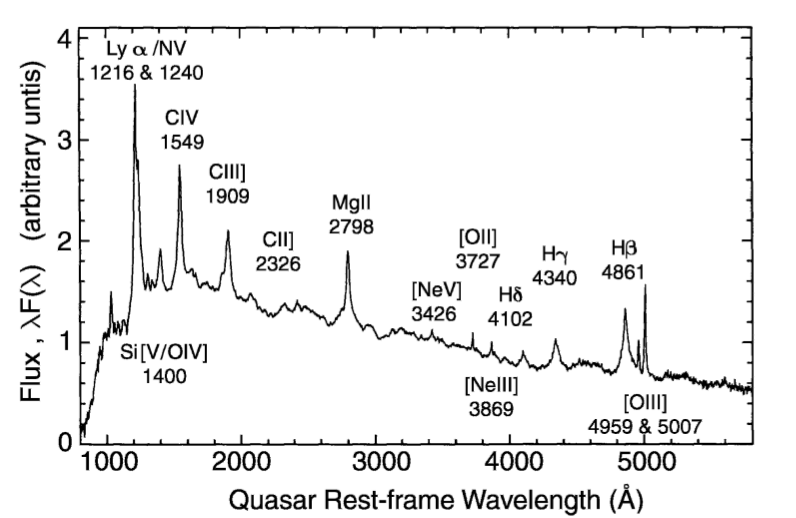
\includegraphics[scale=.3]{./figures/3_AGNs/Espectro_tipico_AGN.png}
\figcaption{\emph{Espectro combinado de varios QSOs, usando el Large Bright Quasar Survey}}\label{fig:Espectro_QSOs}

%---------------------------------------------------------------------
	%M
	\subsection{Propiedades fundamentales de los Cuásares}
	\label{subsec:Fundamental_properties_quasars}
%---------------------------------------------------------------------

Por lo general los cuásares presentan una serie de propiedades que son comunes en varios tipos de AGN's, las propiedades, entre las que se destacan:


- Fueron descubiertos por ser fuentes de radio muy puntual 

- Emite en todas las longitudes de onda, desde el radio a los rayos-X principalmente.

- El flujo de la fuente varía en casi todas las frecuencias y longitudes de onda.

- En general se encuentra que la escala de tiempo de variabilidad es más pequeña y su amplitud más grande, cuando se va ha frecuencias más altas.

- El espectro óptico es muy azul $U-B < -0.3$. La mayoría de los cuásares presentan un corrimiento a rojo alto  $z \lesssim 2$.

- El espectro continuo de un cuásar puede ser descrito por una ley de potencias, sobre un rango de frecuencias muy alto.
%
\begin{align}
S_{\nu} \propto \nu^{-\alpha} \,,
\end{align}
%
 donde $\alpha$ indica el índice espectral. Cuando $\alpha=0$ entonces se tiene un espectro plano, si $\alpha=1$ se tiene un espectro en el cual la misma energía es emitida en cada intervalo de logarítmico de las frecuencias. 


%---------------------------------------------------------------------
	%M
	\subsection{Cuásares, radio fuentes.}
	\label{subsec:}
%---------------------------------------------------------------------

La morfología de los cuásares en el régimen del radio, depende de la frecuencia observada, que a su vez puede presentar un morfología compleja. La morfología del cuásar en una forma simple se puede ver  constituida por varias fuentes extendidas y un núcleo central muy compacto, ver figura (\ref{fig:Lobulos}). En algunas ocasiones es posible observar unas fuentes extendidas llamadas lóbulos, que se extienden de manera simétrica a lo largo de una línea recta. Estos lóbulos se encuentra conectados con el núcleo central por cuenta de los jets, que consiste en la región donde salen despedidas las partículas altamente cargadas proveniente del núcleo. El tamaño del sistema en general puede alcanzar hasta 1 Mpc de largo. La posición óptica coincide con la fuente de radio compacta, cuyo tamaño es mejor a un segundo de arco ($\theta < 1"$).

%---------------------------------------------------------------------
	%
	\subsubsection{Clasificación de las fuentes de radio.}
	\label{subsubsec: clasification_source_radio}
%---------------------------------------------------------------------

Las fuentes de radio extendidas se dividen en dos tipos:

{\it{Fanaroff-Rile Tipo I }} (FR I), son fuentes más brillantes cerca al centro, su brillos superficial decrece hacia el exterior. Poseen una luminosidad típica de $L_{\nu}(1.4GHz)\lesssim 10^{32} erg^{-1} Hz^{-1}$.

{\it{Fanaroff-Rile Tipo II}} (FR II), son fuentes que presentan características contrarias a las (FR I). Su brillo incrementa hacia el exterior, presentan un brillo mayor que las (FR I) $L_{\nu}(1.4GHz)\gtrsim 10^{32} ergs^{-1}Hz^{-1}$, a menudo estas fuentes de radio presentan jets ( Subsección \ref{subsec:Generation_Jets}).

%Los jets, son estructuras que transportan material (partículas cargadas) del núcleo al exterior. Por lo general no son simétricos y a menudo solo es posible ver uno, cuando es posible observar los dos, hay uno más débil que el otro. 


%---------------------------------------------------------------------
	%
	\subsubsection{Radiación Sincrotrón}
	\label{subsubsec: Radiation_synchrotron}
%---------------------------------------------------------------------

La forma espectral y el alto grado de polarización son considerados como consecuencias de la emisión de radio, producida por la radiación sincrotrón \footnote{Radiación producida al someter a partículas cargadas a velocidades muy altas (cercanas a la velocidad de la luz) } de electrones relativistas. Se tiene entonces que los electrones se propagan a través de un campo magnético, a lo largo de un helicoide, produciendo una fuerza de Lorentz, que hace que los electrones sean emitidos a través de la radiación sincrotrón. 

El grado de polarización de un conjunto de electrones depende de la complejidad del campo magnético. Si el campo es homogéneo la medida de polarización observada puede ser mayor al $75\%$. La radiación sincrotrón sigue una ley de potencias si la distribución de energía de los electrones también se comportan como una ley de potencias. 


%*************************************************************************
%AGN Zoo
\section{Tipos de AGN's}
\label{sec:Zoo_AGN's}
%***********************************************************************

Se debe tener muy claro que la diferencia entre los AGN's no radica necesariamente en su forma física. En el contexto de poder "unificar"  los AGN's, su clasificación esta altamente orientada en la dirección de la fuente con la línea de visión del observador. 


%---------------------------------------------------------------------
	%M
	\subsection{Quasi-Stelar Objects.}
	\label{subsec:Quasi-Stelar_Objects}
%---------------------------------------------------------------------

Una pequeña cantidad de cuásares presentan un inusual color azul. La presencia de estos objetos en regiones fuera del rango radio presentan un gran problema para poderlos observar, siendo fuentes muy puntuales.

Las propiedades ópticas de estos objetos son casi indistinguibles de los cuásares. En particular, tienen distribución de energías hacia el azul lo cual es resultado de la forma de búsqueda, además presenta fuertes y anchas líneas de emisión y en general un alto corrimiento al rojo. Por sus propiedades tan parecidas a los cuásares son llamados como {\textit{radio-quiet quasars ó quasi-stelar objects}}, QSOs. Los QSOs son los AGNs que mayor luminosidad, su luminosidad en el núcleo puede ser 1000 veces más que la luminosidad de la galaxia donde se hospeda 

%---------------------------------------------------------------------
	%M
	\subsection{Galaxias Seyfert.}
	\label{subsec:Seyfert_Galaxy}
%---------------------------------------------------------------------

Como se discutió anteriormente las galaxias Seyferts fueron los primeros AGNs descubiertos. La luminosidad de las Seyferts es considerablemente menor que la de los QSOs. Las observaciones en el óptico permiten identificar que las Seyferts son objetos que se encuentra en el centro de las galaxias espirales, presentando un núcleo extraordinariamente brillante, con líneas de emisión  fuertes y anchas.

Se conocen dos tipos de galaxia Seyfert, las Tipo 1 y las Tipo 2. Las Tipo 1 presentan líneas de emisión muy anchas, lo que da un indicio de velocidades de rotación mayor. Las Tipo 2 presentan líneas de emisión más estrechas. Al observar el espectro en el óptico en las Seyfert 1 se identifica que son muy similares a los QSOs. No se conoce una diferencia física entre estos dos objetos, la única diferencia es debida a la luminosidad en sus núcleo. 


%---------------------------------------------------------------------
	%M
	\subsection{Radio Galaxias}
	\label{subsec:Radio_Galaxy}
%---------------------------------------------------------------------

Las radio galaxias son galaxias elípticas que tienen como huésped un AGN. Entre las radio galaxias más conocidas se encuentran Cygnus A y Centuarius A. Al igual que se hizo con las galaxias Seyferts, las radio galaxias también presentan una clasificación debida al ancho de sus  líneas de emisión. Están las radio galaxias de línea ancha (BLRG) y las radio galaxias se línea estrecha (NLRG).

En general los dos tipos de radio galaxias se pueden considerar como radio fuerte Seifert 1 y Seyfert 2, la única diferencia entre Seyfert y radio galaxia es la morfología de la galaxia donde estás hospedadas. 

%---------------------------------------------------------------------
	%M
	\subsection{Variables Opticamente Violentas}
	\label{subsec:Optically_Violently_Variables}
%---------------------------------------------------------------------

Existe otra clase de QSOs, que están caracterizados por su fuerte y rápida variabilidad en su radiación óptica. Son conocidas como OVVs \footnote{Del ingles Optically Violently Variables } (Variables Ópticas Violentas). Estos objetos presentan una variabilidad en escala de tiempo de días. Además de su alta variabilidad, también presentan una muy alta polarización de la luz óptica y fuertes emisiones en radio. Estas fuentes presentan longitudes de onda fuera del rango óptico, aumentando su radiación, con escalas de tiempo más cortas y amplitudes más grandes, a medida que se mueve a frecuencias más altas.  

%---------------------------------------------------------------------
	%M
	\subsection{Objetos BL Lac}
	\label{subsec:BL_Lac}
%---------------------------------------------------------------------

Los BL Lacs son AGNs con una muy fuerte variabilidad en la radiación, como los OVVs, pero sin fuertes líneas de emisión y absorción, haciendo casi imposible la determinación de su corrimiento al rojo $z$. La luminosidad óptica de algunos BL Lacs varia en varias magnitudes si se observa durante periodos de tiempo muy largos.

Algo notable de vez en cuando es el bajón en la luminosidad, a veces se observan líneas de emisión y luego aparece un BL Lac como un OVV. Por este extraño motivo a los OVVs y BL Lacs se les denomina Blazars. Los Blazars son fuentes de radio, con variabilidad violenta y radiación energéticamente fuerte (radiación $\gamma$).


Es importante recordar que la diferencia de los tipos de AGN radica en la dirección de observación en la cual se ve el AGN. En general el AGN es el mismo, solo que esta siendo observado en lugares diferentes que presentan características específicas, como se observa en la figura (\ref{fig:Tipos_AGNs_por_observador}). 

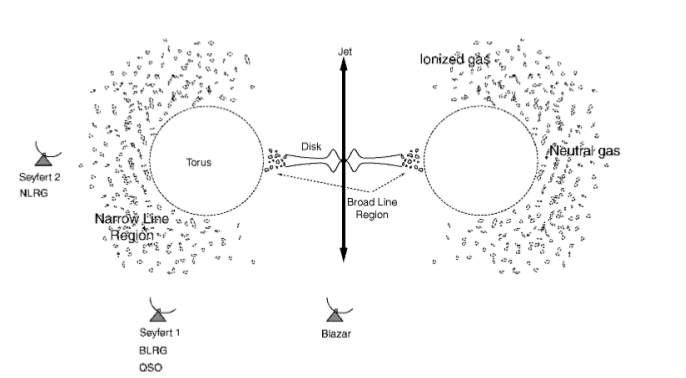
\includegraphics[scale=.5]{./figures/3_AGNs/Clasificacion_AGN}
\figcaption{\emph{Los diferentes tipos de AGNs solo dan información de que lugar del AGN se está observando}}\label{fig:Tipos_AGNs_por_observador}



%*************************************************************************
%AGN Zoo
\section{El Enigma Central: La existencia de un Agujero Negro}
\label{sec:Zoo_AGN's}
%***********************************************************************

En la teoría de los AGNs ha existido una duda sobre el proceder de la energía que estos emanan, en especial ¿ Cómo es producida? Entonces debido a esto, se plantea que dicha energía es originada por un objeto muy masivo en su interior y muy cercano al centro. El objetos propuesto lleva el nombre de Agujero Negro Súper Masivo (SMBH de sus siglas en ingles), objeto altamente compacto que acreta materia de su alrededor. A continuación se presentan una serie de propiedades observacionales de los AGNs que dan pie a la existencia de un SMBH. \\

- Se encuentran fuentes de radio en AGNs que pueden alcanzar un tamaño aproximadamente mayor a 1 Mpc. Usando esta escala de longitud es posible medir el tiempo en que ha estado activa la fuente. Para esta escala de longitud se tiene que el tiempo de vida es mayor a $10^{7}$años.

-La luminosidad de los QSOs es aproximadamente $L_{bol}\sim 10^{47}ergs$. Asumiendo que la luminosidad no cambia sustancialmente durante el tiempo de vida de la fuente, es posible medir la energía total
\begin{align}
E \gtrsim 10^{47} erg/s \times 10^{7}yr \sim 3\times 10^{61}erg\,.
\end{align}

-Para escalas de tiempo de días, se tiene que la luminosidad de los AGNs varia en un $\% 50$. Estas variabilidades permiten encontrar un límite superior para la extensión espacial de la fuente. Para una fuente puntual se tiene que la extensión es $R \lesssim 1$ día luz $\sim3\times10^{15}$cm.


%---------------------------------------------------------------------
	%M
	\subsection{La Existencia de los Agujeros Negros}
	\label{subsec:Why_a_BH}
%---------------------------------------------------------------------

Usando la información observacional expuesta anteriormente y suponiendo que la producción de energía es de naturaleza gravitacional, es posible derivar la energía básica en el AGN. Suponiendo lo anterior la forma clásica más eficiente de generación es por medio de la fusión nuclear. 

La fusión del hidrógeno, produce 8Mev/nucleon. La máxima eficiencia de fusión nuclear es $\epsilon \lesssim 0.81 \%$. Donde $\epsilon$ es la fracción de masa del combustible que es convertido en energía. De acuerdo con 
\begin{align}
E=\epsilon mc^{2}\,,
\end{align}
%
la energía por fusión es $E=3\times10^{61}$. Entonces la masa que produce el combustible necesitaría ser 
\begin{align}
m=\frac{E}{\epsilon c^{2}} \sim 4\times10^{42}g\sim 2\times10^{9}M_{\odot}\,.
\end{align}

Al suponer que la naturaleza de la energía es meramente gravitacional, se tiene entonces que a medida que la materia cae dentro del agujero negro(BH) pierde energía potencial pero adquiere energía cinética . Al convertir la energía cinética en energía interna(calor) que puede ser emitida en forma de radiación.

Sin embargo, los BH no son la única solución simple para las ecuaciones de Einstein. La existencia de un SMBH es posible al conocer la naturaleza de la distribución de masa compacta. También se ha encontrado evidencia observacional que ratifica la existencia de estos objetos super masivos. 

%---------------------------------------------------------------------
	%M
	\subsection{Acreción.}
	\label{subsec:Acretion}
%---------------------------------------------------------------------

A medida que el gas caes hacia un objeto compacto, las partículas de gas pierden energía potencial que a su vez se convierte en cinética. al conocer que el momento angular es finito, se tiene que el gas no puede caer directamente hacia el objeto. A medida que el gas cae, siente una fricción por la interacción con las otras partículas circundantes, lo que se traduce en una transferencia de momentum, que dará como resultado la formación de un disco de acreción perpendicular al momento angular. La fricción en el disco sera la responsable de desacelerar la velocidad de rotación de las partícula haciendo que estas caigan hacia el centro. 

De acuerdo con el teorema del virial, la mitad de la energía potencial se ha cambiado en energía cinética. En este caso, la mitad de la energía se ha convertido en energía de rotación. Así, la mitad de la energía potencial se convirtió en energía interna. 

La energía generada por la viscosidad en el disco, no cuenta con la suficiente energía para poder escapar, pero aun así es capaz de producir calor que genera un engrosamiento en el disco.


%---------------------------------------------------------------------
	%M
	\subsection{Generación de Jets.}
	\label{subsec:Generation_Jets}
%---------------------------------------------------------------------

Los lóbulos radiales son producidos por partículas cargadas eyectadas desde el centro del AGN, a velocidades relativistas. Estas partículas son aceleradas desde el núcleo en dos direcciones opuestas. El impulso es producido por la extracción de energía cinética de rotación del BH a través del mecanismo de Blandford- Znajek. Ver figura (\ref{fig:Modelo_interior_AGN}).% En el disco se encuentra el campo magnético  que está acoplado a este flujo de partículas. 

Al observar un AGN es inevitable ver que los jets producidos son extremadamente delgados y muy rectos. Lo cual implica  que los procesos generadores ocurren muy al interior del disco y el núcleo es el responsable de colimar estos rayos de alta energía. Es importante aclarar que este mecanismo no reproduce los flujos de materia relativista; sin embargo hay una nueva rama que pretende dar solución a este problema. La hidrodinámica es la responsable de reproducir los fenómenos con una mayor precisión, pero con el costo de poder computacional.

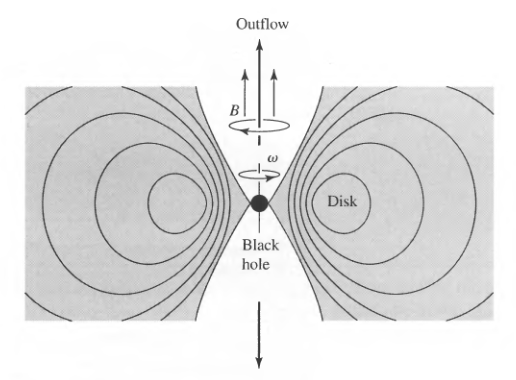
\includegraphics[scale=.4]{./figures/3_AGNs/Jets.png}
\figcaption{\emph{Bosquejo del modelo de la estructura del núcleo del AGN, donde se puede ver el mecanismo de Blandfort- Znajek}}\label{fig:Modelo_interior_AGN}


%---------------------------------------------------------------------
	%M
	\subsection{Formación de Lóbulos.}
	\label{subsec:Formation_lobules}
%---------------------------------------------------------------------

Cuando los jets expulsan las partículas, estas llevan consigo una energía cinética. Estas partículas a medida que se desplazan por el medio interestelar se van desacelerando. Las partículas que van adelante del flujo de materia, son las que más siente la interacción con otras partículas y se van ralentizando, formando un frente de choque. Este frente de choque provoca que las partículas se vaya esparciendo  de forma desordenada generando los lóbulos, como se observa en la figura (\ref{fig:Lobulos}).

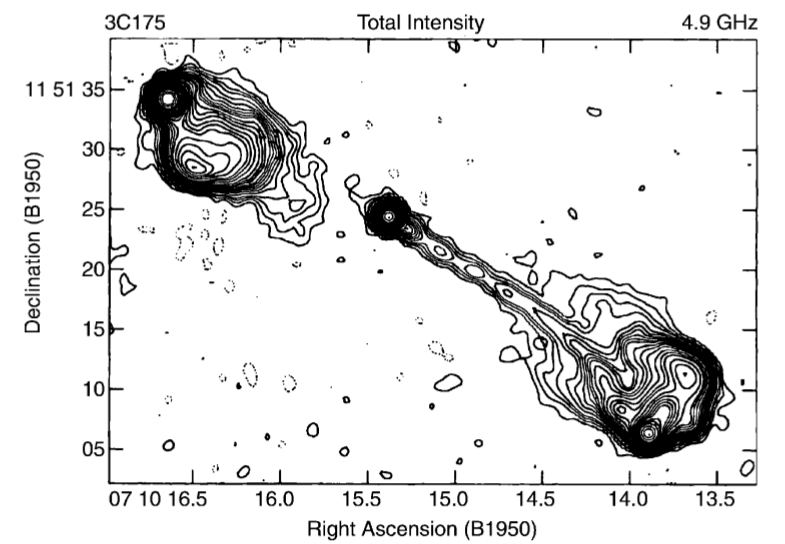
\includegraphics[scale=.3]{./figures/3_AGNs/Lobulos_y_Jets.png}
\figcaption{\emph{Simulación de un AGN. En la parte central se encuentra el BH, los jets son por donde se desplaza la materia y los lóbulos son los grumos donde se aglomera la materia que viene del núcleo.}}\label{fig:Lobulos}


%*********************************************************************
	%M
\section{Modelo Unificado}
\label{sec:Unified_models}
%*********************************************************************

Conforme a todo lo presentado, se puede identificar que los AGNs presentan cierta similitud, pero de igual manera diferencias considerables. Al conocer su naturaleza, se pretende presentar a los AGNs como objetos con morfología equivalentes, pero observados en líneas de visión diferentes. Mirar figura (\ref{fig:Tipos_AGNs_por_observador}).

Como ya se ha dicho y mostrado los AGNs presentan propiedades en común. \\

- Todas los AGNs hospedan un SMBH en su interior. 

- Todos los AGNs tiene un disco de acreción que alimenta el BH.

- Todos los AGNs van a estar caracterizados por la masa del BH $M_{BH}$ y de la rata de acreción $\dot{m}$. $M_{BH}$ permite relacionar la luminosidad máxima del SMBH. 

- La morfología de la galaxia anfitriona también permite clasificar. Las radio galaxias están en galaxias espirales, mientras que las Seyferts en galaxias espirales.





%*************************************************************************

%--------------------------Spin Model ----------------------
%qqqqqqqqqqqqqqqqqqqqqqqqqqqqqqqqqqqqqqqqqqqqqqqqqqqqqqqqqqqqqqqqqqqqqqqqq
%Quote
\begin{savequote}[50mm]
%‘‘El cosmos es todo lo que es, todo lo que fue y todo lo que será. Nuestras 
%más ligeras contemplaciones del cosmos nos hacen estremecer: Sentimos como 
%un cosquilleo nos llena los nervios, una voz muda, una ligera sensación como
%de un recuerdo lejano o como si cayéramos desde gran altura. Sabemos que nos
%aproximamos al más grande de los misterios.’’
%\qauthor{Carl Sagan}
\end{savequote}
%qqqqqqqqqqqqqqqqqqqqqqqqqqqqqqqqqqqqqqqqqqqqqqqqqqqqqqqqqqqqqqqqqqqqqqqqq




%#########################################################################
\chapter{Modelo de Spin.}
\label{cha:Modelo de Spin}














%*************************************************************************

%--------------------- Algoritmo_Modelacion ------------------------
%qqqqqqqqqqqqqqqqqqqqqqqqqqqqqqqqqqqqqqqqqqqqqqqqqqqqqqqqqqqqqqqqqqqqqqqqq
%Quote
\begin{savequote}[50mm]
%‘‘El cosmos es todo lo que es, todo lo que fue y todo lo que será. Nuestras 
%más ligeras contemplaciones del cosmos nos hacen estremecer: Sentimos como 
%un cosquilleo nos llena los nervios, una voz muda, una ligera sensación como
%de un recuerdo lejano o como si cayéramos desde gran altura. Sabemos que nos
%aproximamos al más grande de los misterios.’’
%\qauthor{Carl Sagan}
\end{savequote}
%qqqqqqqqqqqqqqqqqqqqqqqqqqqqqqqqqqqqqqqqqqqqqqqqqqqqqqqqqqqqqqqqqqqqqqqqq




%#########################################################################
\chapter{Algoritmo y Modelación.}
\label{cha:Algoritmo y Modelación}














%***********************************************************************
			
%----------- Clasificación entorno cosmológico-------------------
%qqqqqqqqqqqqqqqqqqqqqqqqqqqqqqqqqqqqqqqqqqqqqqqqqqqqqqqqqqqqqqqqqqqqqqqqq
%Quote
\begin{savequote}[50mm]
%‘‘El cosmos es todo lo que es, todo lo que fue y todo lo que será. Nuestras 
%más ligeras contemplaciones del cosmos nos hacen estremecer: Sentimos como 
%un cosquilleo nos llena los nervios, una voz muda, una ligera sensación como
%de un recuerdo lejano o como si cayéramos desde gran altura. Sabemos que nos
%aproximamos al más grande de los misterios.’’
%\qauthor{Carl Sagan}
\end{savequote}
%qqqqqqqqqqqqqqqqqqqqqqqqqqqqqqqqqqqqqqqqqqqqqqqqqqqqqqqqqqqqqqqqqqqqqqqqq




%#########################################################################
\chapter{Clasificación entorno cosmológico (Cosmic Web)}
\label{cha:cosmic_web}














%***********************************************************************

% --------------------------------------------------------------
%:                  BACK MATTER: appendices, refs,..
% --------------------------------------------------------------

\backmatter


%: ----------------------- bibliography ------------------------



%\bibliographystyle{abbrv}

\bibliographystyle{plainnat}
%\bibliographystyle{abbrvnat}
\bibliography{chapters/references}

%\printnomenclature 
% --------------------------------------------------------------



\end{document}